% Template for PLoS
% Version 1.0 January 2009
%
% To compile to pdf, run:
% latex plos.template
% bibtex plos.template
% latex plos.template
% latex plos.template
% dvipdf plos.template

\documentclass[11pt]{article}

% amsmath package, useful for mathematical formulas
\usepackage{amsmath}
%\usepackage{natbib}
% amssymb package, useful for mathematical symbols
\usepackage{amssymb}
\usepackage{booktabs}
\usepackage{xspace}
% graphicx package, useful for including eps and pdf graphics
% include graphics with the command \includegraphics
\usepackage{graphicx}

%\usepackage{endfloat}
\usepackage{hyperref}

\usepackage{sectsty}
\subsectionfont{\normalsize}
\subsubsectionfont{\mdseries\itshape}

% cite package, to clean up citations in the main text. Do not remove.
\usepackage{cite}
\usepackage{caption}
\usepackage{subcaption}

\usepackage{color} 

% Use doublespacing - comment out for single spacing
\usepackage{setspace} 
\doublespacing


% Text layout
\topmargin 0.0cm
\oddsidemargin 0.5cm
\evensidemargin 0.5cm
\textwidth 16cm 
\textheight 21cm

% Bold the 'Figure #' in the caption and separate it with a period
% Captions will be left justified
\usepackage[labelfont=bf,labelsep=period,justification=raggedright]{caption}

% Use the PLoS provided bibtex style
\bibliographystyle{/Users/stephens/Dropbox/Documents/stylefiles/plos2009}

% Remove brackets from numbering in List of References
\makeatletter
\renewcommand{\@biblabel}[1]{\quad#1.}
\makeatother


% Leave date blank
\date{}

\pagestyle{myheadings}
%% ** EDIT HERE **
\usepackage{enumerate}
\usepackage{multirow} 
\usepackage{url}
\usepackage{xr} %for cross-referencing
%% ** EDIT HERE **
%% PLEASE INCLUDE ALL MACROS BELOW
\newtheorem{algorithm}{Algorithm}
\newtheorem{proposition}{Proposition}
\newtheorem{restateproposition}{Proposition}
\newtheorem{lemma}{Lemma}
\newtheorem{corollary}{Corollary}
\newtheorem{result}{Result}
\newtheorem{note}{Note}
\newtheorem{definition}{Definition}

\def\lfdr{\textit{lfdr}}
\def\lfsr{\textit{lfsr}}
\def\x{\mbf{x}}
\def\y{\mbf{y}}
\def\e{\mbf{e}}
\def\g{\mbf{g}}
\def\p{p}
\def\Yb{\hat{Y}_1^{\text{BAYES}}}
\def\Xperp{X_{1 \perp 0}}
\def\Pperp{P_{1 \perp 0}}
\def\Pperpb{\Pperp^{\text{B}}}
\def \hatd { \widehat{ d } }
\def \dhatin {\hatd^{\mbox{\tiny IN}}}
\def \dhatsw {\hatd^{\mbox{\tiny SW}}}
\def \mvn{\text{MVN}}
\def\mn{\text{MN}}
\def \iw{\text{W}^{-1}}
\def \fp {fastPHASE\ }
\def\bhat{\hat{\beta}}
\def\shat{\hat{s}}
\def\var{\rm Var}
\def\mvr{\text{BMVR}}
\def\bfuni{\text{BF}_\text{uni}}
\def\one{\mbf{1}}
\def\zero{\mbf{0}}
\def\hall{H_{\text{all}}}
\def\pall{\p_{\text{all}}}
\def\bfall{\text{BF}_\text{all}}
\def\bfav{\text{BF}_\text{av}}
\def\gall{\gamma_\text{all}}
\def\limbfall{\bfall^\rightarrow}
\def\limbfav{\bfav^\rightarrow}
\def\limbfgamma{\BF_\gamma^\rightarrow}
\def\sxx{S_{xx}}
\def\syy{S_{yy}}
\def\vyy{V_{yy}}
\def\vyx{V_{yx}}
\def\vxx{{V_{xx}}}
\def\rss{\text{\rm RSS}}
\def\dss{\text{\rm $\Delta$SS}}
\def\U{U}
\def\D{D}
\def\I{I}
\def\luu{L_{UU}}
\def\indep{\perp}
\def\qvalue{{\tt qvalue}\xspace}
\def\locfdr{{\tt locfdr}\xspace}
\def\mixfdr{{\tt mixfdr}\xspace}
\def\ashr{{\tt ashr}\xspace}

\newcommand{\mbf}[1]{\mbox{\boldmath$#1$}} % true mathbf works in math
                                % mode too
\newcommand\height{{\it height}}
\newcommand\weight{{\it weight}}
\def\BF{\text{BF}}


%% END MACROS SECTION
%\externaldocument{plos_one_rev1_suppinfo}

\begin{document}

% Title must be 150 characters or less
\begin{flushleft}
{\Large
\textbf{False Discovery Rates: A New Deal}
}
% Insert Author names, affiliations and corresponding author email.
\\
Matthew Stephens$^{1*}$, 
\\
\bf{1} Department of Statistics and Department of Human Genetics, University of Chicago, Chicago, IL, USA
\\
$\ast$ E-mail: Corresponding mstephens@uchicago.edu
\end{flushleft}

% Please keep the abstract between 250 and 300 words
\section*{Abstract}

We introduce a novel Empirical Bayes approach for large-scale hypothesis testing, including  
estimating False Discovery Rates (FDRs), and estimating effect sizes. Compared with
existing approaches to FDR analysis, the method has two key differences. First, it
assumes that the distribution of the actual (unobserved) effects being tested is unimodal, with a mode at 0.
This ``unimodal assumption" (UA), although natural in many contexts, is very different from assumptions usually made
in FDR analyses, and yields more accurate inferences than existing methods provided that it holds.
The UA also facilitates efficient and robust computation because estimating the unimodal distribution involves solving a simple convex optimization problem.
Second, the method takes as its input two numbers for each test (an effect size estimate, and corresponding standard error),
rather than the one number usually used ($p$ value, or $z$ score). When available, using two numbers instead of one 
helps account for variation in measurement precision across tests. It also facilitates the estimation of actual 
effect sizes, and our approach provides interval estimates (credible regions) for each effect in addition to measures of significance.
To provide a bridge between interval estimates and significance measures we introduce the term ``local false sign rate"
to refer to the probability of getting the sign of an effect wrong, and argue that it is a superior
measure of significance than the local FDR because it is both more generally applicable, and
can be more robustly estimated. Our methods are implemented in an R package {\tt ashr}
available from \href{http://github.com/stephens999/ashr}{http://github.com/stephens999/ashr}. 

% Please keep the Author Summary between 150 and 200 words
% Use first person. PLoS ONE authors please skip this step. 
% Author Summary not valid for PLoS ONE submissions.   
%\section*{Author Summary}

\section*{Introduction}

Since its introduction in 1995 by Benjamini and Hochberg 
\cite{benjamini1995controlling}, the ``False Discovery Rate" (FDR) has quickly established itself
as a key concept in modern statistics, and the primary tool by which most practitioners handle large-scale multiple testing
in which the goal is to identify the non-zero ``effects" among a large number of imprecisely-measured effects.

Here we consider an Empirical Bayes (EB) approach to FDR. This idea is, of course, far from new:
indeed, the notion that EB approaches could be helpful in handling multiple comparisons predates introduction of
the FDR  (e.g.~\cite{greenland1991empirical}). More recently, EB approaches to the FDR
have been extensively studied by several authors, 
especially B.~Efron and co-authors 
\cite{efron2001empirical, efron2002empirical,efron2003robbins,efron2008microarrays,efron2010large}; 
see also \cite{kendziorski2003parametric,newton2004detecting, 
datta2005empirical,muralidharan2010empirical} for example.
So what is the ``New Deal" here? We introduce two simple ideas that are new (at least compared with
existing widely-used FDR pipelines) and can substantially affect
inference. The first idea is to {\it assume that the distribution of effects is unimodal}.  We provide a very simple, fast, and stable computer 
implementation for perfoming EB inference under this assumption, and illustrate how it can improve inference of FDR when the unimodal assumption is correct.  
The second idea is to use two numbers -- effect sizes, and their standard errors -- rather than just one -- $p$ values, or $z$ scores -- 
to summarize each measurement. This idea allows variations in measurement precision to be better accounted for,
 and avoids a problem with standard pipelines that poor-precision measurements can inflate estimated FDR.

In addition to these two new ideas, we highlight a third idea that is old, but which remains under-used in practice:
the idea that it may be preferable to focus on estimation rather than on testing.
In principle, Bayesian approaches can naturally unify testing and estimation into a single framework -- testing is
simply estimation with some positive prior probability that the effect is exactly zero.
However, despite ongoing interest in this area from both frequentist \cite{benjamini2005false} and Bayesian \cite{zhao2012empirical,gelman2012we} 
perspectives, in practice large-scale studies that assess many effects almost invariably focus on testing significance and
controlling the FDR, and not on estimation. To help provide a bridge between FDR and estimation we introduce the term
``local false sign rate" (lfsr), which is analogous to the ``local false discovery rate" (\lfdr) \cite{efron2008microarrays}, but which measures confidence  
in the {\it sign} of each effect rather than confidence in each effect being non-zero. We show that in some settings, particularly those with many discoveries, 
the $\lfsr$ and $\lfdr$ can be quite different, and emphasize benefits of the $\lfsr$, particularly its increased robustness to modeling assumptions. 

%terminology
%``signed discovery" for a discovery (an effect declared to be non-zero) for which the sign of the effect (positive or negative) is declared,
%and correspondingly define the ``false signed discovery rate", or simply ``false sign rate" (FSR), in a natural way. 

%The methods we provide here can address both problems, and we provide results that highlight important benefits of focussing on estimation, and particularly on assessing the correctness of the {\it sign} of the estimated effects, rather than on testing for non-zero effects.

Although we have focussed here on applications to FDR, the idea of performing Empirical Bayes inference by flexibly esimating an underlying unimodal prior distribution
could be useful more generally - for example in shrinkage estimation contexts such as wavelet denoising \cite{donoho:1995}. 
Importantly, our work demonstrates that EB inference under a general unimodal assumption is, if anything, computationally simpler  
than commonly-used more restrictive assumptions -- such as a spike and slab or Laplace prior distribution \cite{johnstone2004needles} --  as well as being more flexible.
Our methods are implemented in an R package, \ashr (for {\bf a}daptive {\bf sh}rinkage in {\bf R}), available at \href{http://github.com/stephens999/ashr}{http://github.com/stephens999/ashr}.
(The name comes from the fact that our EB approach using a unimodal prior naturally results in shrinkage estimation,
and the shrinkage is adaptive to both the amount of signal in the data and the measurement precision of each observation.) 
Code and instructions for reproducing analyses and figures in this paper are at
\href{https://github.com/stephenslab/ash}{https://github.com/stephenslab/ash}.


%Measurement precision will often vary among genes --  for example, log-fold change estimate for highly expressed genes may have greater precision than those for lower-expressed genes -- and one goal  of our methods is to allow for thiis variation. 

%Let $\mu^0_j$ and $\mu^1_j$ denote the mean expression 
%of gene $j$ ($j=1,\dots,J$) in the two conditions, and define $\beta_j:= \mu^0_j - \mu^1_j$ to be the difference. Typically expression
%measurements are made on only a small number of
%samples in each condition - sometimes as few as one
%sample in each condition. Thus the error in estimates
%of $\mu^0_j$ and $\mu^1_j$ is appreciable, and the error
%in estimates of $\beta_j$ still greater.
%

%Many tools have been developed for estimating or controlling the FDR and related quantities \cite{}, and some are widely used.
%Here we present new tools that bring two important ideas to bear on the problem.
%First, these tools are designed to take account of variations in the {\it measurement precision} of different effects, reducing the influence of low-precision measurements.
%For example, in the example of detecting differentially expressed genes, measurements of log fold change for high-expressed genes 
%may have better precision than those for low-expressed genes; by incorporating this information our methods can avoid the tendancy for 
%imprecise measurements at low-expressed genes to dilute the signal at higher-expressed genes.
%Second, our tools explicitly assume that the non-zero effects have a unimodal distribution centered at zero. This assumption 
%is, we argue, often realistic, and comes with considerable benefits, both statistical and computational. 
%Our tools are implemented in an R package \ashr (short for ``Adaptive Shrinkage") and we 
%demonstrate how the incorporation of these two ideas can lead to a substantial reduction in estimated FDRs (or, equivalently,
%a substantial increase in the number of discoveries at a given FDR).  

%Although we motivate our tools by the need to address the FDR problem, our \ashr package, as its name suggests,  provides a general tool for shrinkage estimation. 
%As an important special case, these methods address the "multiple comparisons" setting, where interest usually focuses on which $\beta_j$ can be confidently inferred to be non-zero. Such problems are usually tackled by computing a $p$ value for each $j$, often by applying a $t$ test to $\bhat_j/s_j$,
%and then applying a generic procedure, such as that of \cite{benjamini1995controlling} or \cite{storey2003statistical}, designed to control or
%estimate the false discovery rate (FDR) or the positive FDR \cite{storey.03}. In essence we aim to provide analagous
%generic methods that work directly with two numbers for each 
%measurement $(\bhat_j,s_j$), rather than a single number (e.g.~ the $p$ value, or $t$ statistic). Working with these two numbers has two important benefits: first, it permits estimation and not only testing; second, the 
%uncertainty in each measurement $\bhat_j$ can be more fully accounted for, reducing the impact of ``high-noise" measurements (large $s_j$) that can reduce the effectiveness of a standard FDR analysis. 

\def\df{df}
\def\FDR{\text{FDR}}
\def\fdr{\text{\lfdr}}
\def\FSR{\text{FSR}}
\def\fsr{\text{lfsr}}

 \section*{Methods}

 \subsection*{Model Outine}
 
% Here we consider one setting in which FDR-based methods are widely used:
%an experimenter has measured a large numbers of ``effects", each with an associated
%measurement precision (standard error), 
%and the goal is to identify which of the effects we can declare to be non-zero, with some prescribed level of confidence.
%Although the usual focus of FDR-based methods is on distinguishing zero and non-zero effects,
%here we also focus on providing estimates -- both point estimates and interval estimates -- for these effects.
%This setting arises commonly in many areas of statistics, and particularly in genomics applications.
%For example, in genomics
%a common goal is to identify ``differentially-expressed genes" -- that is, genes
%whose mean expression (activity) level differs in two conditions. Here the ``effect" of interest is the difference in (log) 
%mean expression level between the two conditions, often referred to as the ``log-fold change". 
Here we describe the simplest version of the method, and briefly discuss embellishments we have also implemented.

Suppose that we are interested in the values of $J$ ``effects" $\beta=(\beta_1,\dots,\beta_J)$. For example, in a typical genomics application
that aims to identify differentially expressed genes,  $\beta_j$ might be the difference in the mean (log) expression of gene $j$ in two conditions.
In contexts where FDR methods are applied, interest often focuses on identifying ``significant" non-zero effects;
that is, in testing the null hypotheses $H_j:\beta_j=0$.  Here we tackle both this problem, and the  
more general problem of estimating, and assessing uncertainty in, $\beta_j$.
 
Assume that the available data are estimates $\bhat=(\bhat_1,\dots,\bhat_J)$ of the effects,
and corresponding (estimated) standard errors $\shat=(\shat_1,\dots,\shat_J)$.  Our goal is to compute a posterior distribution for $\beta$ given the observed data $\bhat,\shat$,
which by Bayes theorem can be written as 
\begin{equation}
p(\beta | \bhat, \shat) \propto p(\beta | \shat) p(\bhat | \beta, \shat).
\end{equation}

For $p(\beta | \shat)$ we assume that the $\beta_j$ are independent from a unimodal distribution $g$.
This unimodal assumption (UA) is a key assumption that distinguishes our approach from previous EB approaches to FDR analysis.
A simple way to implement the UA is to assume that $g$ is
a mixture of a point mass at 0 and a mixture of {\it zero-mean} normal distributions:
\begin{align} \label{eqn:beta}
p(\beta | \shat, \pi) & = \prod_j g(\beta_j; \pi), \\   
g(\cdot; \pi) & = \pi_0 \delta_0(\cdot) + \sum_{k=1}^K \pi_k N(\cdot; 0, \sigma_k^2), \label{eqn:mixnorm}
\end{align}
where $N(\cdot; \mu, \sigma^2)$ denotes the density of the normal distribution with mean $\mu$ and variance $\sigma^2$.
Here the mixture proportions $\pi=(\pi_0,\dots,\pi_K)$ are hyper-parameters, which are non-negative and sum to one, and are to be estimated,
while the mixture component standard deviations $\sigma_1,\dots,\sigma_K$ 
represent a large and dense grid of {\it fixed} positive numbers spanning a range from very small to very big (so $K$ is fixed and large). 
(We encourage the reader to think of this grid as becoming infinitely large and dense, as a non-parametric limit,
although of course in practice we use a finite grid -- see Implementation Details.)

For the likelihood $p(\bhat | \beta, \shat)$ we assume  
\begin{equation} \label{eqn:normlik}
p(\bhat | \beta, \shat) = \prod_j N(\bhat_j; \beta_j, \shat_j^2).
\end{equation}
Here, in additional to some conditional independence assumptions, we are 
effectively  assuming that the number of observations used to compute $\bhat_j,\shat_j$ are sufficiently large to justify a normal approximation.

This simple model features both the key ideas we want to emphasize in this paper: the UA is encapsulated in (\ref{eqn:mixnorm}) while
the different measurement precision of different observations is encapsulated in the likelihood (\ref{eqn:normlik}) -- specifically, observations
with larger standard error will have a flatter likelihood, and therefore have less impact on inference.
However, this simple model also has several additional assumptions that can be relaxed. Specifically,
\begin{enumerate}
\item  The use of a mixture of zero-mean normals (\ref{eqn:mixnorm}) implies that $g$ is symmetric about 0.
More flexibility can be obtained by replacing the mixture of normals with mixtures of uniforms [see equation (\ref{eqn:g-general})]; indeed this 
can allow $g$ to approximate {\it any} unimodal distribution. 
\item The model (\ref{eqn:beta}) assumes that the effects are identically distributed, independent of their standard errors $\shat$.
We can relax this to allow for a relationship between these quantities [see (\ref{eqn:beta-alpha})].
\item The likelihood (\ref{eqn:normlik}) effectively assumes that the number of observations used to compute $\bhat_j,\shat_j$ are sufficiently large to justify a normal approximation. We can generalize this likelihood using a $t$ likelihood [see (\ref{eqn:tlik})].
\end{enumerate}
These embellishments are detailed in Detailed Methods.
Of course there remain limitations that are harder to relax, most notably the independence and conditional independence assumptions encapsulated in our model
(which are also made by most existing EB approaches to this problem). Correlations among tests certainly arise in practice, either due to genuine correlations
in the system of study, or due to unmeasured confounders, and their potential to impact results of an FDR analysis is important to consider
whatever analysis methods are used: see \cite{efron2007correlation,leek:2007} for relevant discussion.

%We assume that the observations $\bhat$ are conditionally independent given $\beta,\shat$, and that the distribution of
%$\bhat_j$ depends only on the corresponding $\beta_j,\shat_j$, so
%\begin{equation}
%p(\bhat | \beta, \shat) = \prod_j p(\bhat_j | \beta_j, \shat_j).
%\end{equation}
%Initially we assume that the number of observations used to compute $\bhat_j,\shat_j$ are sufficiently large to justify a normal approximation,
%\begin{equation} \label{eqn:normlik}
%p(\bhat_j | \beta_j, \shat_j) =  N(\bhat_j; \beta_j, \shat^2_j),
%\end{equation}
%where $N(\cdot; \mu,\sigma^2)$ denotes the density of a normal distribution with mean $\mu$ and variance $\sigma^2$.
%
%We assume that the (unobserved) effects $\beta_j$ come from some distribution $g$, which is to be estimated, and which we write 
%as a mixture of null and alternative components:
%\begin{equation} \label{eqn:betaj0}
%g(\cdot) = \pi_0 \delta_0(\cdot) + (1-\pi_0) g_1(\cdot)
%\end{equation}
%where $\pi_0$ denotes the proportion of effects that are null, $\delta_0(\cdot)$ denotes a point mass at 0, and $g_1(\cdot)$ denotes the distribution of the non-zero $\beta_j$.
%We also assume that (given $g$) the $\beta_j$ are independent, and independent of $\shat$ (a point we return to later), so
%\begin{equation} \label{eqn:beta-iid}
%p(\beta | \shat) = \prod_j g(\beta_j).
%\end{equation}
%
%Our key further assumption, which distinguishes our approach from previous EB approaches to FDR analysis, is that $g_1$ is unimodal,
%with a mode at 0. One simple way to implement this ``Unimodal Assumption" (UA)  is
%to use a mixture of zero-mean normal distributions:
%\begin{equation} \label{eqn:mixnorm}
%g_1(\cdot) = \sum_{k=1}^K w_k N(\cdot; 0, \sigma_k^2)
%\end{equation}
%where $N(\cdot; \mu,\sigma^2)$ denotes the density of a normal distribution with mean $\mu$ and standard deviation $\sigma$.
%Here the $w_k$ are non-negative mixture weights that sum to $1$ and are to be estimated, and the component standard deviations $\sigma_1,\dots,\sigma_K$ 
%represent a large and dense grid of fixed positive numbers spanning a range from very small to very big (so $K$ is fixed and large).
% The symmetry of the normal distribution implies that (\ref{eqn:mixnorm}) is not only unimodal, but also symmetric about zero. We introduce
% more flexible alternatives based on using mixtures of uniform distributions, and further details (such as choice of gridpoints $\{\sigma_k:k=1,\dots,K\}$) below. 
% 
% Substituting (\ref{eqn:mixnorm}) for $g_1$ in (\ref{eqn:betaj0}), and defining $\pi_k := (1-\pi_0)w_k$ for $k=1,\dots,K$ (and also $\sigma_k:=0$, and $N(\cdot;0,0):=\delta_0(\cdot)$)
% yields a notationally-convenient form for $g$, with hyperparameters $\pi:=(\pi_0,\pi_1,\dots,\pi_K)$ whose elements are non-negative and sum to 1:
% \begin{equation} \label{eqn:g}
% g(\cdot; \pi) = \sum_{k=0}^K \pi_k N(\cdot; 0, \sigma_k^2).
% \end{equation}
% 
% Putting all this together, and making the dependence on hyperparameters $\pi$ explicit, we have:
% \begin{align} \label{eqn:betaj}
% p(\beta | \shat, \pi) & = \prod_j g(\beta_j; \pi), \\  \label{eqn:normlik2}
% p(\bhat | \beta, \shat, \pi) &= \prod_j N(\bhat_j; \beta_j, \shat_j^2), 
% \end{align}
% with $g$ given by the mixture of normals $(\ref{eqn:g})$.
 

\subsection*{Fitting the model}
 
In words, the model above assumes that the effects $\beta_j$ are independent and identically distributed from a mixture of zero-centered normal distributions, and 
each observation $\bhat_j$ is a noisy measurement of $\beta_j$ with standard error $\shat_j$.
Together, these assumptions imply that the observations $\bhat_j$ are also independent observations, each from a mixture of normal distributions:
\begin{equation} \label{eqn:marginallik}
p(\bhat | \shat, \pi) =   \prod_j  [\sum_{k=0}^K \pi_k N(\bhat_j; 0, \sigma_k^2 + \shat_j^2)],
\end{equation}
where we define $\sigma_0:=0$.

The usual EB approach to fitting this model would involve two simple steps:
\begin{enumerate}
\item Estimate the hyper-parameters $\pi$ by maximizing the likelihood $L(\pi)$, given by (\ref{eqn:marginallik}), yielding $\hat{\pi} := \arg \max L(\pi)$.
\item Compute quantities of interest from the conditional distributions $p(\beta_j | \bhat, \shat, \hat{\pi})$. For example, the evidence
against the null hypothesis $\beta_j=0$ can be summarized by $p(\beta_j \neq 0 | | \bhat, \shat,\hat{\pi})$.
\end{enumerate}
Both steps 1 and 2 are very straightforward. Step 1 is a convex optimization problem, and can be solved quickly and reliably using interior point methods \cite{boyd2004convex,koenker2013convex}. (Alternatively a simple EM algorithm can be used, and we found this to perform adequately for moderate-sized problems, say $J<2000$). And the conditional distributions $p(\beta_j | \bhat_j, \shat_j,\hat{\pi})$ in Step 2 are analytically available, each a mixture of a point mass on zero and $K$ normal distributions.
(The simplicity of step 1 is due to our use of a fixed grid for $\sigma_k$ in (\ref{eqn:mixnorm}), instead of estimating $\sigma_k$,
which may seem more natural but is not straightforward when $\shat_j$ varies among $j$. This simple device may be useful in other applications.)

Here we slightly modify this usual procedure: instead of obtaining $\hat\pi$ by maximizing the likelihood, we maximize a penalized
likelihood [see (\ref{eqn:penalty})], where the penalty encourages $\hat\pi_0$ to be as big as possible whilst remaining consistent with the observed data. 
We introduce this penalty because in FDR applications it is considered desirable to avoid underestimating $\pi_0$ so as to avoid underestimating the FDR. 

Our {\tt R} package implementation typically takes about $~20$ seconds on a modern laptop for $p=100,000$, and scales linearly with $J$. 

\subsection*{The local False Discovery Rate and local False Sign Rate}

As noted above, the posterior distributions $p(\beta_j | \bhat, \shat, \hat{\pi})$ have a simple analytic form.
In practice it is common, and desirable, to summarize these distributions to convey the ``significance" of each observation $j$.
One natural measure of the significance of observation $j$ is its ``local FDR" \cite{efron2008microarrays}, which is
the probability, given the observed data, that effect $j$ would be a false discovery, if we were to declare it a discovery.
In other words it is the posterior probability that $\beta_j$ is actually zero:
\begin{equation} \label{eqn:fdr}
\fdr_j := \Pr(\beta_j =0  |  \bhat, \shat, \hat{\pi}).
\end{equation}


The $\lfdr$, like most other measures of significance (e.g. $p$ values and $q$ values), is rooted in the hypothesis testing paradigm which focuses on 
whether or not an effect is exactly zero. This paradigm is popular, despite the fact that many statistical practitioners have argued that it is often inappropriate because
the null hypothesis $H_j: \beta_j=0$ is often implausible. For example, Tukey  (\cite{tukey1991philosophy}) argued that
``All we know about the world teaches us that the effects of $A$ and $B$ are always different -- in some decimal place -- for any $A$ and $B$. Thus asking `Are the effects different?' is foolish." Instead, Tukey suggested (\cite{tukey1962future}, p32,) that one should address
\begin{quote}
...the more meaningful question: ``is the evidence strong enough to support a belief that the observed difference has the correct sign?"
\end{quote}
Along the same lines, Gelman and co-authors \cite{gelman2000type, gelman2012we} suggest  
focussing on ``type S errors", meaning errors in sign, rather than the more traditional type I errors.

Motivated by these suggestions, we define the ``local False Sign Rate" for effect $j$, $\lfsr_j$, to be the probability that we
would make an error in the sign of effect $j$ if we were forced to declare it either positive or negative. Specifically,
\begin{equation} \label{eqn:lfsr}
\lfsr_j := \min[ p(\beta_j \geq 0| \bhat, s), p(\beta_j \leq 0| \hat\pi, \bhat, s) ].
\end{equation}
To illustrate, suppose that 
\begin{gather*}
p(\beta_j < 0| \bhat, s, \hat\pi)=0.95, \\
p(\beta_j =0| \bhat, s, \hat\pi) = 0.03, \\
p(\beta_j >0| \bhat, s, \hat\pi) = 0.02.
\end{gather*} 
Then 
from (\ref{eqn:lfsr}) $\lfsr_j=\min(0.05,0.98)=0.05$ (and, from (\ref{eqn:fdr}), $\lfdr_j=0.03$). This $\lfsr$ corresponds to the fact that, given these results, 
our best guess for the sign of $\beta_j$ is that it is negative, and the probability that this guess is wrong would be $0.05$. 

As our notation suggests, $\lfsr_j$ is intended to be compared and contrasted with $\lfdr_j$: whereas small values of $\lfdr_j$ indicate that we can be {\it confident that $\beta_j$ is non-zero}, 
small values of $\lfsr_j$ indicate that we can be {\it confident in the sign of $\beta_j$}. 
Of course, being confident in the sign of an effect logically implies that we are confident it is non-zero, and
this is reflected in the fact that $\lfsr_j \geq \lfdr_j$ 
(this follows from the definition because both the events $\beta_j \geq 0$
and $\beta_j \leq 0$ in (\ref{eqn:lfsr}) include the event $\beta_j=0$).
In this sense, as a measure of ``significance", $\lfsr$ is more conservative than $\lfdr$. More importantly, as we illustrate in Results,
$\lfsr$ can be substantially more robust to modeling assumptions than $\lfdr$.

From these ``local" measures of significance, we can also compute average error rates over subsets of observations
$\Gamma \subset \{1,\dots,J\}$. For example,   
\begin{equation} \label{eqn:FDRhat}
\widehat\FDR(\Gamma):= (1/|\Gamma|) \sum_{j \in \Gamma} \fdr_j. 
\end{equation}
estimates the FDR we would obtain if we were to declare all tests in $\Gamma$ significant.
And 
\begin{equation} \label{eqn:qvalue}
q_j := \widehat \FDR(\{k: \fdr_k \leq \fdr_j\}) 
\end{equation}
provides a measure of significance analogous to Storey's $q$ value \cite{storey.03}.

%Because our methods involve explicitly modelling effects $\beta_j$, rather than 
%$p$ values or $z$ scores, they can provide estimates of the local false sign rates.

%Indeed, even in settings where some
%$\beta_j$ are exactly zero, separately identifying which are positive and which negative may be useful. For example, when identifying differentially expressed genes,
%analysts will often separate the genes that are ``upregulated" from those that ``downregulated" in a condition.

\subsection*{Related work}

\subsubsection*{Previous approaches focussed on FDR}

Among previous methods that explicitly consider the FDR and related quantities,
our work here seems most naturally compared with the EB methods of \cite{efron2008microarrays} and \cite{muralidharan2010empirical}
 (implemented in the R packages \locfdr and \mixfdr respectively) and with the widely-used methods from  \cite{storey.03} (implemented in the R package \qvalue), which although not formally an EB approach, shares some elements in common.
  %Here we highlight the key differences between our approach and these three existing approaches.

There are two key differences between our approach and all of these three existing methods. First, 
whereas these existing methods summarize the information on $\beta_j$ by a single number -- either a $z$ score (\locfdr and \mixfdr), or a $p$ value (\qvalue) -- 
we instead work with two numbers ($\bhat_j,\shat_j$). Here we are building on \cite{wakefield:2009}, who develops Bayesian tests 
for individual null hypotheses using these two numbers, using the normal approximation \ref{eqn:normlik}; see also \cite{efron1993bayes}.
Using two numbers instead of one clearly has the potential to be more informative, and indeed, results later (Figure \ref{fig:goodpoor}) illustrate 
how it can improve performance by taking better account of variation in measurement precision among observations.
%(And in the special case where $\shat_j$ are equal for all $j$, our approach essentially comes down to the same thing as these existing methods.)
% Or more generally Section xx illustrates the potential practical effects

%allows for different modelling assumptions to be compared through likelihood comparisons.
Second, our unimodal assumption (UA) that the effects are unimodal about zero is quite different from assumptions made by $\qvalue, \locfdr$ or $\mixfdr$.
Indeed, $\locfdr$ assumes that all $z$ scores near 0 are null (Efron calls this the Zero Assumption; ZA), which implies that 
under the alternative hypothesis the distribution of $z$ scores has {\it no mass at 0}; this contrasts strikingly with the UA, which implies that this distribution has its peak at 0! 
Similarly, $\qvalue$ assumes that all $p$ values near 1 are null,
which is the same as the ZA because $p$ values near 1 correspond to $z$ scores near 0. And although \mixfdr does not formally make the ZA,
we have found that in practice, with default settings, the results often approximately satisfy the ZA (due, we believe, to the default choice of penalty term $\beta$ described in \cite{muralidharan2010empirical}). Thus, not only do these existing methods not make the UA, they actually make assumptions that are, in some sense, as different
from the UA as they can be. 

Given that the UA and ZA are so different, it seems worth discussing why we generally favor the UA. 
Although the UA will not apply to all situations, we believe that it will often be reasonable, especially in FDR-related contexts
that have traditionally focussed on rejecting the null hypotheses $\beta_j=0$. This is because if ``$\beta_j=0$" is a plausible null hypothesis,  
it seems reasonable to expect that ``$\beta_j$ very near 0" is also plausible. Further, it seems reasonable to expect that larger effects become
decreasingly plausible, and so the distribution of the effects will be unimodal about 0. To paraphrase Tukey, ``All we know about the world teaches us that large effects are rare, whereas small effects abound."
We emphasize that the UA relates to the distribution of {\it all} effects, and not only the {\it detectable} effects (i.e.~those that are significantly different from zero). It is very likely that the distribution of {\it detectable} non-zero effects will be multimodal, with one mode for detectable positive effects and another for detectable negative effects, and the UA does not contradict this. 

%Tukey "peri-null"

%Interestingly, although the unimodal assumption seems natural, much previous related work on estimating False Discovery Rates  
%has assumed, either explicitly or implicitly, that the distribution of effects is multimodal - see Figure \ref{fig:ZA}. 

In further support of the UA for FDR applications, we note that almost all analogous work in sparse regression models make the UA for the regression coefficients -- 
common choices of uni-modal distribution being the spike and slab, Laplace, $t$, normal-gamma, normal-inverse-gamma, or horseshoe priors \cite{carvalho2010horseshoe}.
These are all less flexible than the approach we take here, which provides for general uni-modal distributions, and 
it may be fruitful to apply our methods to the regression context; indeed see \cite{moser:2015} for work in this vein. 
The UA assumption on regression coefficients is directly analagous to our UA here, and so its
widespread use in the regression context supports its use here. 

Alternatively, we could motivate the UA by its effect on point estimates, which is to ``shrink" the estimates towards the mode - 
such shrinkage is desirable from several standpoints for improving estimation accuracy. Indeed most model-based approaches to shrinkage
make parametric assumptions that obey the UA (e.g. \cite{johnstone2004needles}).

Finally, the UA also has a considerable practical benefit: it yields simple algorithms that are both computationally
and statistically stable (see Results).

\subsubsection*{Other work}

There is also a very considerable literature that does not directly focus on the FDR problem, but which involves similar ideas and methods. 
 Among these, a paper about deconvolution \cite{cordy1997deconvolution} is most similar, methodologically, to our work here:
indeed, this paper includes all the elements of our approach outlined above, except for the point mass on 0 and corresponding penalty term.
This said, the focus is very different: \cite{cordy1997deconvolution} focuses entirely on estimating $g$, whereas our primary focus is on estimating $\beta_j$.
Also, they provide no software implementation.  More generally, the related literature is too large to review comprehensively, but relevant key-words include ``empirical bayes", ``shrinkage", ``deconvolution", ``semi-parametric", ``shape-constrained", and ``heteroskedastic". Some pointers to recent papers in which other relevant
citations can be found include \cite{xie2012sure, sarkar:2014, koenker2014convex}. Much of the literature focusses on the homoskedastic case (i.e. $\shat_j$ all equal) whereas we allow for heteroskedasticity. And much of the recent shrinkage-oriented literature focuses only on point estimation of $\beta_j$, whereas for FDR-related applications measures of uncertainty are essential. Several recent papers consider more flexible non-parametric assumptions on 
$g$ than the UA assumption we make here. In particular, \cite{jiang2009general,koenker2014convex} consider the unconstrained non-parametric maximum likelihood
estimate (NPMLE) for $g$. These methods may provide alternatives to our approach in settings where the UA assumption is considered too restrictive. However, the  NPMLE for $g$ is a discrete distribution, which will induce a discrete posterior distribution on $\beta_j$, and so although the NPMLE
may perform well for point estimation, it may not adequately reflect uncertainty in $\beta_j$, and some regularization on $g$ may be necessary.
Indeed, one way of thinking about the UA is as a way to regularize $g$.




%The conditional distributions $p(\beta_j | \bhat, \shat, \hat{\pi})$ 
%encapsulate uncertainty in $\beta_j$, combining information across {\it all} observations 
%$j=1,\dots,J$. Specifically, the combining of the information occurs through estimation of
%$\pi$, which involves all of the data. Importantly, when estimating $\pi$ our approach accounts for
%the precision of each measurement through the likelihood (\ref{eqn:normlik}). For example, 
%observations with a large $\shat_j$ have an essentially flat likelihood, and so have little effect on estimation of $\pi$, and
%corresondingly little effect on the estimated FDR of other observations. 
%We highlight this because it contrasts with approaches that model the $p$ values or $z$ scores directly: observations with large $\shat_j$ will tend to produce 
%$p$ values with approximately $U[0,1]$ distribution, and $z$ scores with an approximately $N(0,1)$ distribution, under both the null and the alternative hypothesis (assuming
%that the effect $\beta_j$ is small compared with $\shat_j$). Such noisy observations therefore do affect inference; specifically they add to the
%estimated weight of the null component $\pi_0$, and inflate estimates of the FDR. 
%Because of this our approach can take better account of the informativeness of each measurement, as illustrated in Results below.


\def\dt{\text{dt}}

%
%assume that the likelihood $L(\beta) := p(D | \beta)$ can be approximated by 
%$\hat{L}(\beta) := \prod_j \hat{L}_j(\beta_j)$ where
% $\hat{L}_j(\beta_j) := p(\bhat_j | \beta_j, \shat_j)$ is given by 
%  \begin{equation} \label{eqn:lik}
% \hat{L}_j(\beta_j) \propto \dt_\nu(\bhat_j; \beta_j, \shat_j)
% \end{equation}
% where $\dt_\nu(\cdot; \mu,\sigma)$ denotes the density of the generalized $t$ distribution on $\nu$ degrees of freedom with mean $\mu$ and scale parameter $\sigma$ (i.e. the density of $\mu+\sigma T_\nu$). In the special case $\nu \rightarrow \infty$ this corresponds, of course, to a normal approximation to the likelihood:
%  \begin{equation} \label{eqn:normlik}
% \hat{L}_j(\beta_j) \propto N(\bhat_j; \beta_j, \shat_j).
% \end{equation}
%which, in light of (\ref{eqn:betahat}), is equivalent to
 % \begin{equation} \label{eqn:lik2}
% L(\beta_j) \propto p(\bhat_j | \beta_j, \shat_j).
 %\end{equation}
 
  

%The $t$ likelihood (\ref{eqn:lik}) can derived from an assumption of conditional independence of the data on each effect given the true effects, plus two additional assumptions: a) $\bhat_j, \shat_j$ contain most of the information about $\beta_j$ in the data $D_j$ (i.e. they are ``approximately sufficient" for $D_j$); and b) $\shat_j$ alone contains little information about $\beta_j$. The former (a) suggests the approximation $\hat{L}_j(\beta_j) \propto p(\bhat_j, \shat_j | \beta) = p(\bhat | \beta, \shat_j) p(\shat_j | \beta)$, while the latter (b) suggests assuming that $p(\shat_j|\beta_j)$ does not depend on $\beta_j$. Putting these two together yields $\hat{L}_j(\beta_j) \propto p(\bhat_j | \beta, \shat_j)$. If $\bhat_j, \shat_j$ are not sufficient for $D_j$ then there is some loss of efficiency in making this approximation, but all Bayesian inferences remain valid provided they are interpreted as conditional on $\bhat_j,\shat_j$, rather than conditional on $D_j$. See \cite{johnson:2008} and \cite{wakefield:2009} for more general discussion and examples of Bayesian inference based on summary statistics. 

%This likelihood approximation can be motivated by assuming that i) $\bhat$
% $(\bhat_j -\beta_j)/\shat_j | \shat_j$ has a $T_\nu$ distribution, and then writing
% $p(D_j | \beta_j) = p(\bhat_j, \shat_j | \beta) = $ as sufficient for $\beta$. 
% 


%Alternatively (\ref{eqn:lik}) could be considered definitional for $\bhat_j,\shat_j$: that is, choose $\bhat_j,\shat_j,\nu$ such that (\ref{eqn:lik}) holds. 

%While has parallels with approaches like \cite{efron2008microarrays, sun2007oracle}
 %that model the $Z$ scores $Z_j = \bhat_j/\shat_j$ as normally distributed under the null, 
%there is an important difference: here, 

%The choice of normal likelihood seems natural, and indeed it can be motivated in multiple ways. For example, we can write $p(\bhat_j, \shat_j | \beta_j) = p(\bhat_j | \shat_j, \beta_j)p(\shat_j | \beta_j)$. Now, if we are willing to assume that $\shat_j$ alone contains no information about $\beta_j$, or equivalently that $p(\shat_j | \beta_j)$ does not depend on $\beta_j$, then $L(\beta_j) \propto p(\bhat_j | \shat_j, \beta_j)$, and if $\bhat_j | \shat_j, \beta_j \sim N(\beta_j, \shat_j^2)$, as is often asymptotically the case, then we obtain the likelihood (**) above.



\section*{Results}

We compare results of \ashr with existing FDR-based methods implemented
in the R packages \qvalue (v2.1.1), \locfdr (v1.1-8), and \mixfdr (v1.0, from \href{https://cran.r-project.org/src/contrib/Archive/mixfdr/}{https://cran.r-project.org/src/contrib/Archive/mixfdr/}).  
In all our simulations we assume that the test statistics follow the expected theoretical distribution under the null, and we indicate this
to \locfdr using {\tt nulltype=0} and to \mixfdr using {\tt theonull=TRUE}. Otherwise all packages were used with default options.


\subsection*{Effects of the Unimodal Assumption}

Here we consider the effects of making the UA. To isolate these effects we consider the simplest case, where every observation has the same
standard error, $s_j=1$ and all methods are provided that information. That is,
$\bhat_j | \beta_j \sim N(\beta_j,1)$ and $\shat_j=s_j=1$. In this case the $z$ scores $z_j:=\bhat_j/\shat_j=\bhat_j$, so modelling the $z$ scores is the same as modelling the $\bhat_j$, and so the only difference between our method and methods like $\locfdr$ and $\mixfdr$ are in how they estimate $g$.

To briefly summarize the results in this section:
\begin{enumerate}
\item The UA can produce very different inferences compared with the ZA made by existing methods.
\item The UA can yield conservative estimates of the proportion of true nulls, $\pi_0$, and hence conservative estimates of $\lfdr$ and $\FDR$.
\item The UA results in a stable procedure, both numerically and statistically, and is somewhat robust to deviations from unimodality.
\end{enumerate}

\subsubsection*{The UA and ZA can produce different inferences}

\begin{figure}
\center 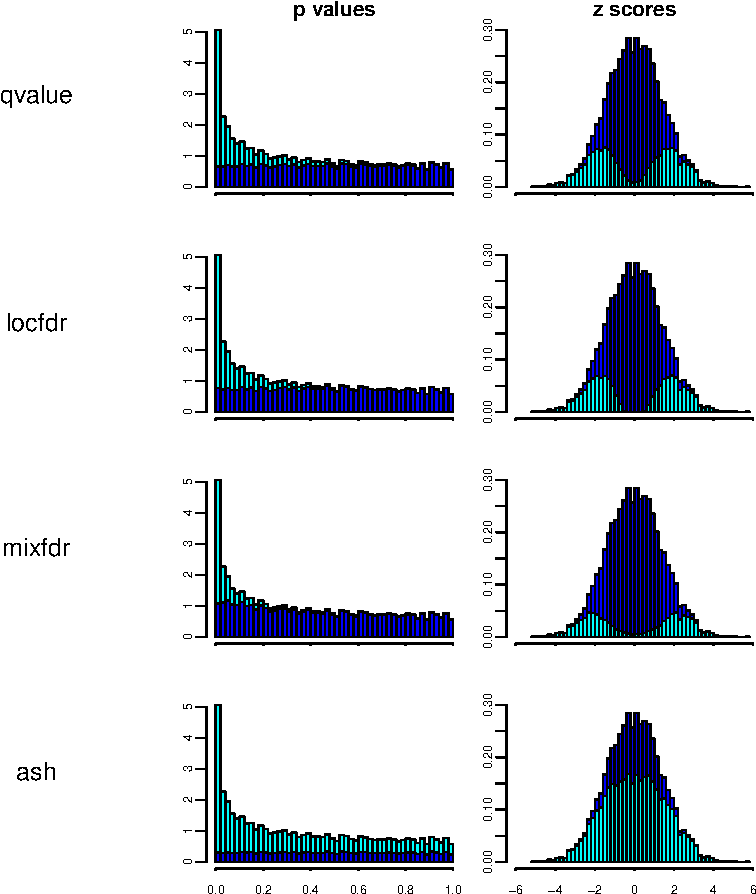
\includegraphics[height=6in]{../analysis/figure/makefig_FDReg.Rmd/decomp_ZA-1.pdf}
\caption{Illustration that the unimodal assumption (UA) in \ashr can produce very different results from existing methods.
The figure shows, for a single simulated dataset, the way different methods decompose $p$ values (left) and $z$ scores (right) into a null component (dark blue) and an alternative component (cyan). In the $z$ score space the alternative distribution is placed on the bottom to highlight the differences in its shape among methods.
The three existing methods (\qvalue, \locfdr, \mixfdr) all effectively make the Zero Assumption, which results in a ``hole" in the alternative $z$ score distribution around 0.
In contrast the method introduced here (\ashr) makes the Unimodal Assumption -- that the effect sizes, and thus the $z$ scores, have a unimodal distribution about 0 -- which yields a very different decomposition. (In this case the \ashr decomposition is closer to the truth: the data were simulated under a model where all of the effects are non-zero, so the ``true" decomposition would make everything cyan.)} \label{fig:ZA}
\end{figure}

To illustrate the different inferences from the UA and ZA we show results for a single
dataset simulated with the true effects $\beta_j \sim N(0,1)$ (so with $s_j=1$, $\bhat_j  \sim N(0,2)$). Note that none of the effects are truly null,
but nonetheless there are many $p$ values near 1 and $z$ scores near 0 (Figure \ref{fig:ZA}).  We used each of the methods
\qvalue, \locfdr, \mixfdr and \ashr to decompose the $z$ scores ($z_j = \bhat_j$), or their corresponding $p$ values, into null and alternative components.
The results (Figure \ref{fig:ZA}) illustrate the clear difference between the existing methods and our method. The effects of the ZA made by \qvalue and \locfdr
are visually clear, producing a ``hole"  in the alternative $z$ score distribution around 0. Although \mixfdr does not formally make the ZA, its decomposition
exhibits a similar hole. In contrast, due to the UA, the alternative $z$ score distribution for \ashr is required to have a mode at 0, 
effectively ``filling in" the hole.  (Of course the null distribution also has a peak at 0, and the local fdr 
 under the UA is still smallest for $z$ scores that are far from zero -- i.e. large $z$ scores remain the ``most significant".)
 
Figure \ref{fig:ZA} may also be helpful in understanding the interacting role of the UA and the penalty term (\ref{eqn:penalty}) that attempts to make $\pi_0$ as ``large as possible" while remaining consistent with the UA. Specifically, consider the panel of Figure \ref{fig:ZA} that shows \ashr's decomposition of $z$ scores, and imagine increasing $\pi_0$ further. This would increase the null component (dark blue) at the expense of
the alternative component (light blue). Because the null component is $N(0,1)$, and so is biggest at 0, this would eventually create a ``dip" in the light-blue histogram at 0. The role of the penalty term is to push the dark blue component as far as possible, right up to (or, to be conservative, just past) the point where this dip appears. In contrast the ZA pushes the dark blue component until the light-blue component {\it disappears} at 0. See \href{https://stephens999.shinyapps.io/unimodal/unimodal.Rmd}{https://stephens999.shinyapps.io/unimodal/unimodal.Rmd} for an interactive
demonstration.

 \subsubsection*{The UA can produce conservative estimates of $\pi_0$}

The illustration in Figure \ref{fig:ZA} suggests that the UA will produce smaller estimates of $\pi_0$ than the ZA.
Consequently \ashr will estimate smaller $\lfdr$s and FDRs than existing methods that make the ZA. 
This is desirable, provided that these estimates remain conservative: that is,
provided that $\pi_0$ does not underestimate the true $\pi_0$ and $\lfdr$ does not underestimate the true $\lfdr$.
The penalty term (\ref{eqn:penalty}) aims to ensure this conservative behavior. To check its effectiveness
we performed simulations under various alternative scenarios (i.e. various distributions for the non-zero effects, which we denote $g_1$), and values
for $\pi_0$. The alternative distributions are shown in Figure \ref{fig:altdens}, with details in Table \ref{table:scenarios}.
They range from a ``spiky" distribution -- where many non-zero $\beta$ are
too close to  zero to be reliably detected, making reliable estimation of $\pi_0$ essentially impossible -- to a much
flatter distribution, which is a normal distribution with large variance (``big-normal") -- where most non-zero $\beta$ are easily detected
making reliable estimation of $\pi_0$ easier. We also include one asymmetric distribution (``skew"), and one clearly bimodal distribution (``bimodal"),
which, although we view as generally unrealistic, we include to assess robustness of \ashr~to deviations from the UA.



% How do these differences influence estimates of the FDR? To address this, note that  -- in this simple case where the 
% $\shat_j$ are all identical --  the primary driver of differences in FDR estimates among methods is {\it differences in their estimates
% of $\pi_0$}. To see why, observe that, given an estimate $\hat\pi_0$ for $\pi_0$, equation (\ref{eqn:FDRest}) provides a 
% strikingly natural non-parametric estimate for the FDR (provided the denominator is not very small). Thus, 
% although the methods considered here differ from one another in many ways, having estimated $\pi_0$
% they should, if sensible, produce estimates of FDR that agree closely with (\ref{eqn:FDRest}). And, indeed, limited
% empirical checks suggest that this is indeed the case (\href{https://www.github.com/stephens999/ash/examples/qvalue.nonp.rmd}).
% 

%Thus, differences in FDR estimates among methods are driven primarily by differences in their estimates of $\pi_0$,
% and so to assess differences in FDR estimates among methods we focus on assessing differences in estimates of $\pi_0$.
%Figure \ref{fig:ZA} suggests that, compared with the ZA, the UA will tend to reduce the estimate of $\pi_0$. 
%At the same time, provided the UA holds, we hope still to provide ``conservative" estimates of $\pi_0$ (that is,
%overestimates of $\pi_0$, which will yield overestimates of the FDR).




\begin{figure} 
\begin{center}
\begin{subfigure}{\textwidth}
	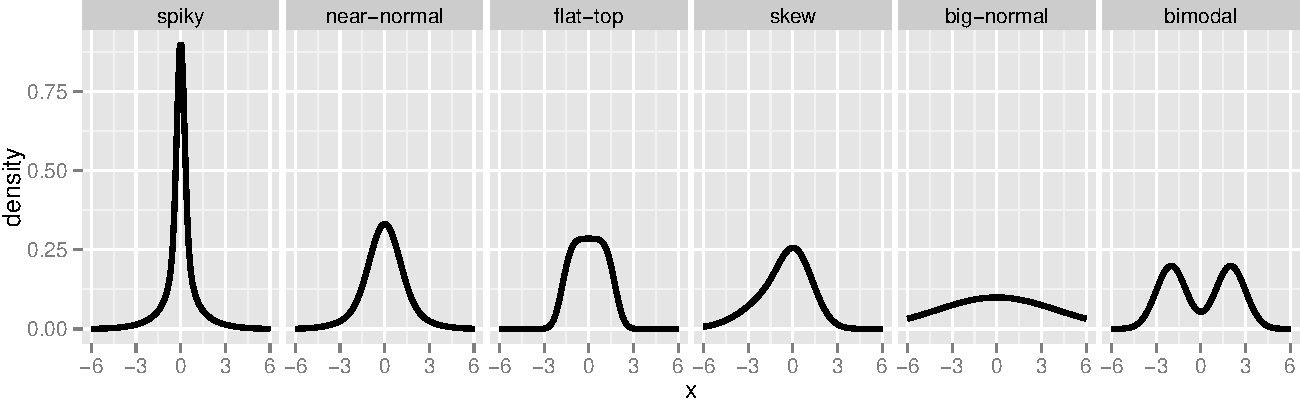
\includegraphics[width=\textwidth]{../analysis/figure/plot_egdens.Rmd/scenario_density-1.pdf} 
	\caption{Densities of non-zero effects, $g_1$, used in simulations.} \label{fig:altdens}
\end{subfigure}
\begin{subfigure}{\textwidth}
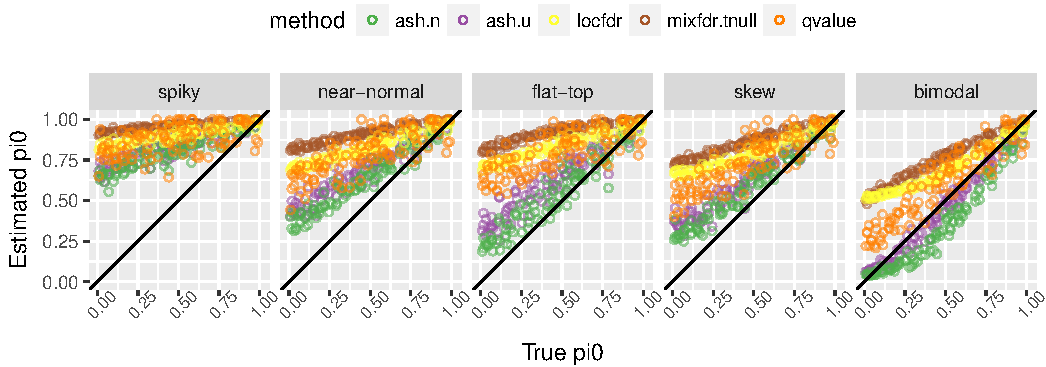
\includegraphics[width=\textwidth]{../analysis/figure/plot_pi0est.Rmd/plot_pi0est-1.pdf} 
\caption{Comparison of true and estimated values of $\pi_0$. When the UA holds all methods yield conservative (over-)estimates for $\pi_0$, with \ashr being least conservative, and hence most accurate. When the UA does not hold (``bimodal" scenario) the \ashr estimates are slightly anti-conservative.} \label{fig:pi0sims}
\end{subfigure}
\begin{subfigure}{\textwidth}
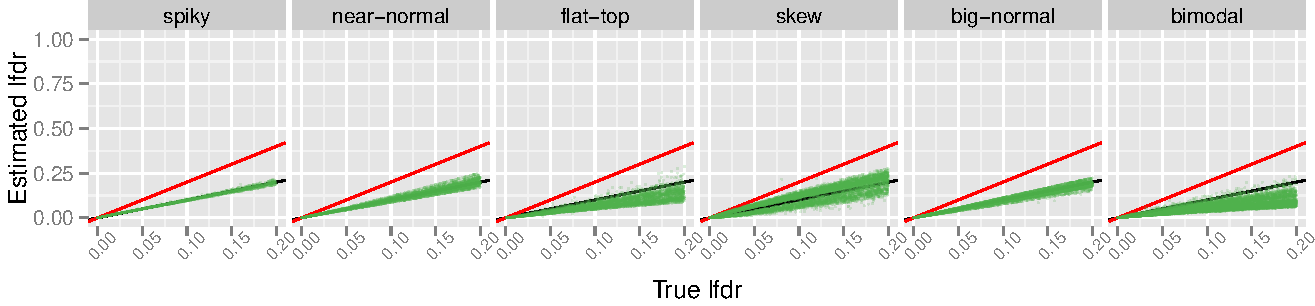
\includegraphics[width=\textwidth]{../analysis/figure/plot_lfsr.Rmd/plot_lfdr-1.pdf} 
\caption{Comparison of true and estimated $\lfdr$ from \ashr (ash.n). Black line is $y=x$ and red line is $y=2x$. Estimates of $\lfdr$ are conservative when UA holds, due to conservative estimates of $\pi_0$.} \label{fig:lfdr}
\end{subfigure}
\begin{subfigure}{\textwidth}
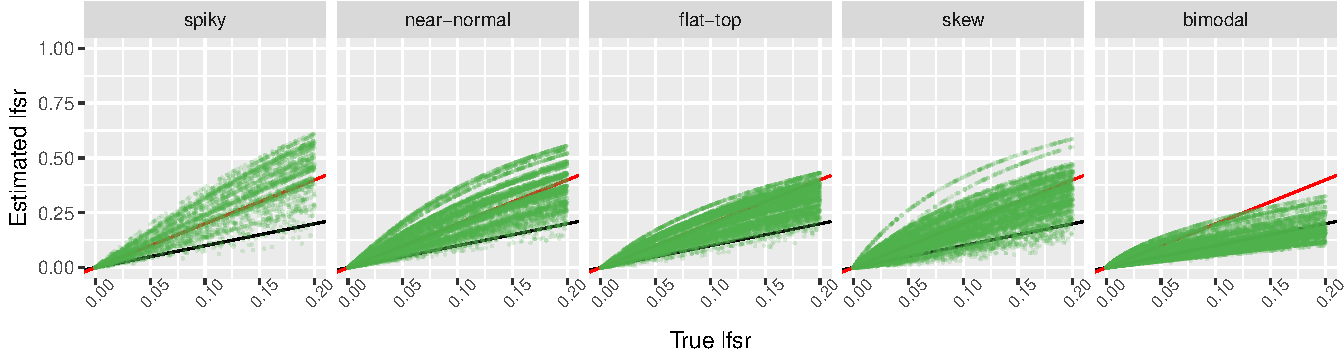
\includegraphics[width=\textwidth]{../analysis/figure/plot_lfsr.Rmd/plot_lfsr-1.pdf} 
\caption{As in c), but for $\lfsr$ instead of $\lfdr$. Estimates of $\lfsr$ are consistently less conservative than $\lfdr$ when UA holds, and also less anti-conservative in bimodal scenario.}  \label{fig:lfsr}
\end{subfigure}
\end{center}
\caption{Results of simulation studies (constant precision $s_j=1$).}
\end{figure}


For each simulation scenario we simulated 100 independent data sets, each with $J=1000$ observations. For each data set we simulated
data as follows:
\begin{enumerate}
\item Simulate $\pi_0  \sim U[0,1]$.
\item For $j=1,\dots,J$, simulate $\beta_j \sim \pi_0 \delta_0 + (1-\pi_0) g_1(\cdot)$.
\item For $j=1,\dots,J$, simulate $\bhat_j | \beta_j \sim N(\beta_j,1)$.
\end{enumerate}
%Thus these simulations assume the same
%precision $1$ for each measurement, and for all methods this precision is assumed known (i.e. $\shat_j=1$).

Figure \ref{fig:pi0sims} compares estimates of $\pi_0$ from \qvalue, \locfdr, \mixfdr and \ashr ($y$ axis) with the true values ($x$ axis). 
For \ashr we show results for $g_1$ modelled as a mixture of normal components (``ash.n") 
and as a mixture of symmetric uniform components (``ash.u"). (Results using the asymmetric uniforms, which we refer to
as ``half-uniforms", and denote ``ash.hu" in subsequent sections, are here generally similar to ash.u and omitted to avoid over-cluttering figures.)
The results show that \ashr provides the smallest more accurate, estimates for $\pi_0$, while remaining conservative
in all scenarios where the UA holds. When the UA does not hold (``bimodal" scenario) the \ashr estimates can be slightly anti-conservative.
We view this as a minor concern in practice, since we view such a strong bimodal scenario as unlikely in most applications where FDR methods
are used. (In addition, the effects on $\lfsr$ estimates turn out to be relatively modest; see below). 


%\subsubsection{The UA produces less conservative estimates of $\pi_0$}
%
%The data in Figure \ref{fig:ZA} were simulated assuming that the true effects are standard normal, $\beta_j \sim N(0,1)$,
%and so all effects are non-zero and no nulls hold. This scenario is rather different
%from the ``mostly null" scenarios that originally motivated FDR methods, where most tests are null,
%and relatively few are non-null. It could be argued that the existing FDR methods are not well adapted to the 
%``mostly non-null"
%scenario, and we would agree! On the other hand, the distribution of $p$ values
%in Figure \ref{fig:ZA} looks like data that, before this work, we would have been happy to apply
%existing FDR methods to. Further, we believe that both ``mostly non-null" and ``mostly null" scenarios likely occur in practical applications.
%Thus it seems desirable to have methods that perform well in both cases, and this is
%an important feature of the methods we introduce here.
%
%TODO: put FDRs on graph? Simulate with 50\% null?


\subsubsection*{The $\lfsr$ is more robust than \lfdr}

The results above show that \ashr can improve on existing methods in producing smaller, more accurate, 
estimates of $\pi_0$, which will lead to more accurate estimates of FDR.
Nonetheless, in many scenarios \ashr continues
to substantially over-estimate $\pi_0$ (see the ``spiky" scenario for example). 
This is because these scenarios include 
an appreciable fraction of ``small non-null effects" that are essentially indistinguishable from 0, making accurate
estimation of $\pi_0$ impossible. Put another way, and as is well known, $\pi_0$ is not identifiable:
 the data can effectively provide an upper bound on plausible values of $\pi_0$,
but not a lower bound (because the data cannot rule out that everything is non-null, but with minuscule effects).
To obtain conservative behavior we must estimate $\pi_0$ by this upper bound, which can
be substantially larger than the true value. 

Since FDR-related quantities depend quite sensitively on $\pi_0$, the consequence of this 
overestimation of $\pi_0$ is corresponding overestimation of FDR (and $\lfdr$, and $q$ values).
To illustrate, Figure \ref{fig:lfdr} compares the estimated $\lfdr$ from ash.n with the true value (computed using
Bayes rule from the true $g_1$ and $\pi_0$). As predicted, $\lfdr$ is overestimated, especially in scenarios which involve many
non-zero effects that are very near 0 (e.g.~the spiky scenario with $\pi_0$ small) where
$\pi_0$ can be grossly overestimated.  
(Of course other methods will be similarly affected by this: those that more grossly overestimate $\pi_0$, will more grossly overestimate $\lfdr$ and FDR/$q$-values.)

The key point we want to make here is estimation of $\pi_0$, and the accompanying identifiability issues,
 become substantially less troublesome if we use the local false sign rate $\lfsr$ (\ref{eqn:lfsr}), rather than $\lfdr$, to measure significance. 
 This is essentially because $\lfsr$ is less sensitive to the estimate of $\pi_0$.
To illustrate, Figure \ref{fig:lfsr} compares the estimated $\lfsr$ from ash.n with the true value: although the estimated $\lfsr$ continue to
be conservative, overestimating the truth, the overestimation is substantially less pronounced than for the $\lfdr$, especially for
the ``spiky" scenario. Further, in the bi-modal scenario, the anti-conservative behavior is less pronounced in $\lfsr$ than $\lfdr$.

Note that, compared with previous debates regarding testing, 
this section advances an additional reason for focussing on the sign of the effect, rather than just testing whether it is 0. 
In previous debates authors have argued against testing whether an effect is 0
because it is {\it implausible that effects are exactly 0}. Here we add that {\it even if one believes
that some effects may be exactly zero}, it is still better to focus on the sign, because generally {\it the data are more informative about that question}
and so inferences are more robust to, say, the inevitable mis-estimation of $\pi_0$.
To provide some intuition, consider an observation with a $z$ score of 0. The $\lfdr$ of this observation can range from 0 (if $\pi_0=0$)
to 1 (if $\pi_0=1$). But, assuming a symmetric $g$, the $\lfsr>0.5$ whatever the value of $\pi_0$, because the observation $z=0$ says
nothing about the sign of the effect.
Thus, are two reasons to use the $\lfsr$ instead of the $\lfdr$: it answers a question that is more generally meaningful (e.g. it applies
whether or not zero effects truly exist),  and estimation of $\lfsr$ is more robust. 
 
Given that we argue for using $\lfsr$ rather than $\lfdr$, one might ask whether we even need a point mass on zero in our analysis.
Indeed, one advantage of the $\lfsr$ is that it makes sense even if no effect is exactly zero. And, 
if we are prepared to assume that no effects are exactly zero, then removing the point mass 
yields smaller and more accurate estimates of $\lfsr$ when that assumption is true (Figure \ref{fig:lfsr-nn}). 
However, there is ``no free lunch":  if in fact some effects are exactly zero
then the analysis with no point mass will tend to be anti-conservative, underestimating $\lfsr$ (Figure \ref{fig:lfsr-s}). 
We conclude that {\it if} ensuring a ``conservative" analysis is important then one must allow for a point mass at 0. 

\subsubsection*{The UA helps provide reliable estimates of $g$}

An important advantage of our EB approach based on modelling the effects $\beta_j$, rather than $p$ values or $z$ scores, is that it
can estimate the {\it size} of each effect $\beta_j$.
Specifically, it provides a posterior distribution for each $\beta_j$, which can be used
to construct interval estimates for $\beta_j$ and address question such as ``which effects exceed $T$'', for any 
threshold $T$.
%Importantly, because the posterior distribution for $\beta_j$ depends on the ``prior" effect-size distribution $g$, which is estimated from {\it all} the observations,
%this posterior reflects information from all the observations and not only from the observation $\bhat_j$. 
%In our case, because we assume $g$ to be unimodal about zero, this prior always ``shrinks" the posterior distributions
%towards zero, with the strength of the shrinkage being estimated from the data.
Further, because the posterior distribution is, by definition,
conditional on the observed data, interval estimates based on posterior distributions are also valid Bayesian inferences for any subset of the effects that have
been selected based on the observed data. This kind of ``post-selection" validity is much harder to achieve in the frequentist paradigm.
In particular the posterior distribution solves the (Bayesian analogue of the) ``False Coverage Rate" problem posed by
\cite{benjamini2005false} which \cite{efron2008microarrays} summarizes as follows: ``having applied FDR methods to select a set of nonnull cases,
how can confidence intervals be assigned to the true
effect size for each selected case?". \cite{efron2008microarrays} notes the potential for EB approaches to tackle this problem,
and \cite{zhao2012empirical} consider in detail the case where the non-null effects are normally distributed.
%but also notes the difficulties of implementing a stable general algorithm. 

The ability of the EB approach to provide valid ``post-selection" interval estimates is extremely attractive in principle.
But its usefulness in practice
depends on reliably estimating the distribution $g$. Estimating $g$ is a ``deconvolution problem",
which are notoriously difficult in general. Indeed, Efron emphasizes
the difficulties of implementing a stable general algorithm, noting in his rejoinder
``the effort foundered on practical difficulties involving the perils of deconvolution... Maybe I am trying
to be overly nonparametric ... but it is hard to imagine a
generally satisfactory parametric formulation..." (\cite{efron2008microarrays} rejoinder, p46).
Our key point here is that the UA greatly simplifies the deconvolution problem.
While not meeting Efron's desire for an entirely general nonparametric approach, we believe 
that the UA can handle many cases of practical interest. 

To illustrate this, Figure \ref{fig:egcdf} compares the
estimated $g$ from \ashr  with that from \mixfdr which does not make the UA 
(and which models $g$ as a mixture of $J$ normal distributions, with $J=3$ by default).
The greater reliability of estimates afforded
by the UA is immediately apparent. In particular the estimated cdf from \mixfdr often has an almost-vertical
segment at some non-zero location, indicative of a concentration of density in the estimated $g$ at that location. 
The UA prevents this kind of ``irregular" behavior, effectively requiring $g$ to be somewhat smooth.
While the UA is not the only way to achieve this, we find it an attractive, simple and effective approach.

Interestingly, even in the ``bimodal" scenario $\ashr$ 
is visually more accurate than \mixfdr: although \mixfdr is capable, in principle, of fitting the multiple modes of $g$, it does not do this well here. 
Possibly the noise level here is sufficiently large to make reliable estimation of the multiple modes difficult. 
Indeed, in multi-modal simulations where the multiple modes are sufficiently well-spaced
to be clearly visible in the observed $\bhat$, \mixfdr fits these modes 
(\href{http://stephenslab.github.io/ash/analysis/check_mixfdr_lownoise.html}{http://stephenslab.github.io/ash/analysis/check\_mixfdr\_lownoise.html}). 
Of course, we would not advocate the UA in settings where multi-modality is 
clearly visible in the observed $\bhat$.

We note one caveat on the accuracy of estimated $g$: due to the penalty term (\ref{eqn:penalty}) \ashr tends to systematically
overestimate the mass of $g$ near zero. On careful inspection, this is apparent in Figure \ref{fig:egcdf}: the estimated cdf is generally below the true cdf just to the left of zero,
and above the true cdf just to the right of zero. Averaging the cdf over many replicates confirms this systematic effect (Figure \ref{fig:egcdf}b),
and applying our methods without the penalty term removes this systematic effect, although at the cost of sometimes 
under-estimating $\pi_0$ (Figure \ref{fig:egcdf}c). 

\begin{figure}[h!] 
\begin{subfigure}{\textwidth}
	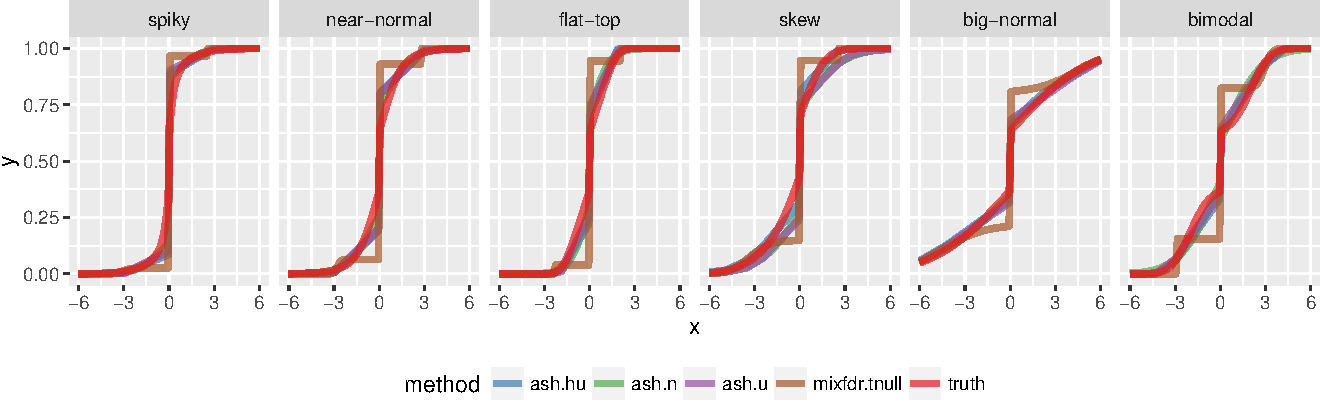
\includegraphics[height=2in]{../analysis/figure/plot_cdf_eg.Rmd/egcdf-1.pdf}
	\caption{Example estimated cdfs for single data sets compared with truth. The unimodal assumption made by the ash methods effectively regularizes estimates compared with \mixfdr.}
\end{subfigure}
\begin{subfigure}{\textwidth}
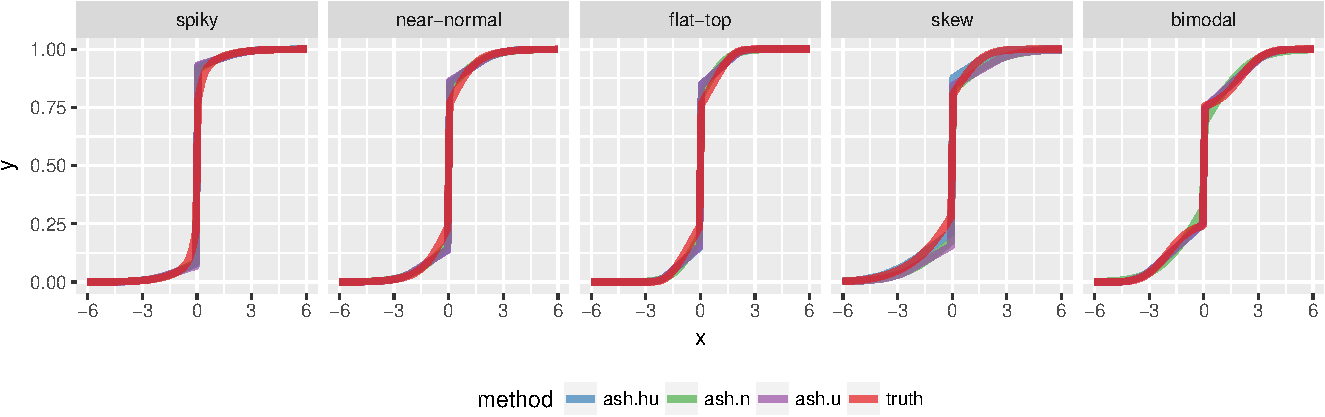
\includegraphics[height=2in]{../analysis/figure/plot_cdf_eg.Rmd/mean_cdf-1.pdf}
\caption{Average estimated cdfs across $\sim10$ data sets compared with truth; methods here use penalty (\ref{eqn:penalty}) so $\pi_0$ is systematically overestimated.}
\end{subfigure}
\begin{subfigure}{\textwidth}
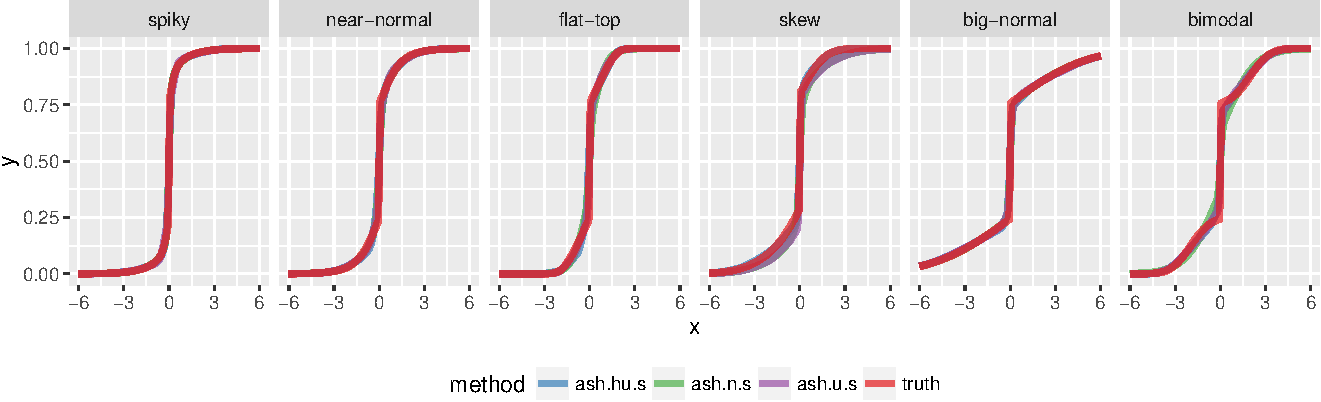
\includegraphics[height=2in]{../analysis/figure/plot_cdf_eg.Rmd/mean_cdf_nopen-1.pdf}
\caption{Average estimated cdfs across $\sim10$ data sets compared with truth; methods here do not use penalty (\ref{eqn:penalty}) so $\pi_0$ is not systematically overestimated. Systematic differences from the truth in ``skew" and ``bimodal" scenarios highlight the effects of model mis-specification.}
\end{subfigure}
\caption{Comparisons of estimated cdfs of $g$ and true cdf of $g$. See Figure \ref{fig:pi0sims} for simulation scenarios.} \label{fig:egcdf}
\end{figure}


%making the UA provides an attractive and simple way to achieve estimating $g$  large
%subset of cases of interest (those where the UA can reasonably be assumed to hold).

%In practice, the utility of the posterior distributions noted above depends primarily on the accuracy
%of the estimate of the distribution $g(\cdot)$. 
 
 %quote from efron rejoinder , p46:
%Morris� Section 3 is especially pertinent. His formula
%for p(?|z) is related to my discussion of the
%Benjamini�Yekutieli False Coverage Rate method in
%Section 7, particularly (7.2)�(7.4). Originally I had
%hoped to develop an empirical Bayes method for estimating
%such models, but the effort foundered on practical
%difficulties involving the perils of deconvolution.
%Section 6 on the �one-group model� is the ugly duckling
%of the current paper, but it bears on some important
%points raised in the discussion. Figure 7 concerns
%a fuzzy version of simultaneous hypothesis testing,
%where, as in Morris� hospital example, the usual singlepoint
%null hypotheses seem unequal to the task. The
%development from (6.6) onwards, particularly (6.12),
%bears on the possibility of nonnormal null distributions,
%and is about as far as I can go in answering Professors
%Rice and Spiegelhalter�s penultimate question.
%With g(?) a normal distribution, model (6.1) returns
%us to the realm of Stein estimation, the scene of my
%happy collaborations with Carl Morris. I continue to
%be surprised at how much harder bumpy, nonnormal
%models like (7.1) are to deal with. James�Stein estimation
%works fine with, say, N = 10 component problems,
%while the Robbins� form of empirical Bayes appropriate
%to (7.1) seems to require hundreds or thousands.
%The information calculations in Efron (2008)
%reinforce this gloomy assessment. Maybe I am trying
%to be overly nonparametric in constructing the empirical
%Bayes Fdr estimates, but it is hard to imagine a
%generally satisfactory parametric formulation for (6.1).
%Or perhaps it is just that hypothesis testing is more demanding
%than estimation.
%My Note: (6.1) is the general model (mu \sim g()).
%7.1 is the case where the effects are a mixture of zero and N(-3,1).

\subsubsection*{Calibration of posterior intervals}

To quantify the effects of errors in estimates of $g$ we examine the calibration of the resulting posterior distributions (averaged over 100 simulations in each Scenario). 
Specifically we examine the empirical coverage of nominal lower 95\% credible bounds for a) all observations; b) significant negative discoveries; c) significant positive discoveries.  We examine only lower bounds because the results for upper bounds follow by 
symmetry (except for the one asymmetric scenario). We separately examine positive and negative discoveries because the lower bound plays a different role
in each case: for negative discoveries the lower bound is typically large and negative and limits how big (in absolute value) 
the effect could be; for positive discoveries the lower bound 
is positive, and limits how small (in absolute value) the effect could be. Intuitively, the lower bound for negative discoveries depends on the accuracy of $g$ in its tail,
whereas for positive discoveries it is more dependent on the accuracy of $g$ in the center.

The results are shown in Table \ref{tab:coverage}.  Most of the empirical coverage rates are in the range 0.92-0.96 for nominal coverage of 0.95, which we view
as adequate for practical applications. The strongest deviations from nominal rates are noted and discussed in the table captions.

% As noted above, the penalty term (\ref{eqn:penalty}) causes systematic over-estimation of the mass of $g$ near 0,  which one would expect to overshrink interval estimates towards zero. 
%The effect of overshrinking on the left tail area is different for ``negative discoveries" and ``positive discoveries": for negative discoveries the lower credible bound is negative and overshrinking (moving it too far towards zero) makes the left tail too big; conversely, for positive discoveries, the lower confidence bound is positive, and  
%overshrinking (moving it too far towards zero) makes the tail too small. In the context of reliably identifying ``large" effects we might worry more about under-shrinkage, 
%and be prepared to put up with some overshrinkage to avoid it. 

%Coverage rates are given in:
%\href{file:///Users/stephens/Dropbox/Documents/git/ash/dsc-shrink/investigate_cdf.html}


%Note - this could probably be solved by making the small components symetric - the idea is that the asymetry only comes in with the tail.

\begin{table}[!ht]
\begin{subtable}{\textwidth}
	\centering% latex table generated in R 3.2.3 by xtable 1.7-4 package
% Sun Jan 24 15:11:55 2016
\begin{tabular}{rrrrrrr}
  \toprule  & spiky & near-normal & flat-top & skew & big-normal & bimodal \\ 
  \midrule ash.n & 0.90 & 0.94 & 0.95 & 0.94 & 0.96 & 0.96 \\ 
  ash.u & 0.87 & 0.93 & 0.94 & 0.93 & 0.96 & 0.96 \\ 
  ash.hu & 0.88 & 0.93 & 0.94 & 0.94 & 0.96 & 0.96 \\ 
   \bottomrule \end{tabular}


	\caption{All observations. Coverage rates are generally satisfactory, except for the extreme ``spiky" scenario. This is due to the penalty term (\ref{eqn:penalty}) which tends to cause over-shrinking towards zero. Removing this penalty term produces coverage rates closer to the nominal levels for uniform and normal methods (Table \ref{tab:nopen}). Removing the penalty in the half-uniform case is not recommended (see Appendix).}
\end{subtable}

\begin{subtable}{\textwidth}
\centering% latex table generated in R 3.3.2 by xtable 1.8-2 package
% Mon Jan  2 09:27:03 2017
\begin{tabular}{rrrrrrr}
  \toprule  & spiky & near-normal & flat-top & skew & big-normal & bimodal \\ 
  \midrule ash.n & 0.93 & 0.94 & 1.00 & 0.94 & 1.00 & 0.98 \\ 
  ash.u & 0.88 & 0.90 & 0.93 & 0.91 & 1.00 & 0.94 \\ 
  ash.hu & 0.87 & 0.87 & 0.92 & 0.93 & 1.00 & 0.94 \\ 
   \bottomrule \end{tabular}


\caption{``Significant" negative discoveries. Coverage rates are generally satisfactory, except for the uniform-based methods in the spiky and near-normal scenarios,
and the normal-based method in the flat-top scenario. These results likely reflect inaccurate estimates of the tails of $g$ due to a disconnect between the tail of $g$ and the component distributions in these cases. For example, the uniform methods sometimes substantially underestimate the length of the tail of $g$ in these long-tailed scenarios, 
causing over-shrinkage of the tail toward 0.}
\end{subtable}

\begin{subtable}{\textwidth}
\centering% latex table generated in R 3.2.3 by xtable 1.7-4 package
% Sun Jan 24 15:11:53 2016
\begin{tabular}{rrrrrrr}
  \toprule  & spiky & near-normal & flat-top & skew & big-normal & bimodal \\ 
  \midrule ash.n & 0.94 & 0.94 & 0.94 & 0.86 & 0.95 & 0.96 \\ 
  ash.u & 0.93 & 0.93 & 0.93 & 0.84 & 0.95 & 0.95 \\ 
  ash.hu & 0.92 & 0.92 & 0.93 & 0.92 & 0.95 & 0.95 \\ 
   \bottomrule \end{tabular}


\caption{``Significant" positive discoveries. Coverage rates are generally satisfactory, except for the symmetric methods under the asymmetric (``skew") scenario. }
\end{subtable}

\caption{Table of empirical coverage for nominal 95\% lower credible bounds} \label{tab:coverage}
\end{table}


%
%\subsubsection*{Reverse asymptotics}
%
%Note that if observation precisions are all similar and most observations are null then all the methods likely to give similar results?
%
%Note: we'd like to make sure it behaves ok in the case where most observations are null.
%Perhaps simulate with 999 null and 1 alternative?
%Also maybe look at performance for small sample sizes - e.g. n=1?
%
%Note that, even though the exact value of the point mass $\pi_0$ cannot, in general, be reliably estimated, the actual underlying distribution $g$ 
%can be quite accurately estimated from the data, provided we assess accuracy by a metric that is not sensitive to $\pi_0$: for example
%by measuring the difference between the true and estimated cumulative distribution function (cdf). See supplementary Figure \ref{} for examples.
%


\subsection*{Differing measurement precision across units}

 We turn now to the second important component of our work: allowing for varying
 measurement precision across units. The key to this is the use of a likelihood,
 (\ref{eqn:normlik}) or (\ref{eqn:tlik}), that explicitly incorporates the measurement precision (standard error) of each $\bhat_j$.
 
  To illustrate, we conduct a simulation where half the measurements are quite precise (standard error $s_j = 1$), and the other half are very poor
 ($s_j=10$).  In both cases,
we assume that half the effects are null
and the other half are normally distributed with standard deviation 1:
\begin{equation}
p(\beta) = 0.5 \delta_0(\beta) + 0.5 N(\beta; 0,1).
\end{equation}
In this setting, the poor-precision measurements $(s_j=10)$ tell us very little, and any sane analysis should effectively ignore them. 
 However, this is not the case in standard FDR-type analyses (Figure \ref{fig:goodpoor}). This is because the poor measurements 
 produce $p$ values that are approximately uniform  (Figure \ref{fig:goodpoor}a), 
 which, when combined with the good-precision measurements, dilute the overall signal (e.g. they reduce the density of $p$ values near 0).
 This is reflected in the results of FDR methods like $\qvalue$ and $\locfdr$:
the estimated error rates ($q$-values, or $\lfdr$ values) for the good-precision observations increase when the low-precision observations are included in the analysis
(Figure \ref{fig:goodpoor}b). In contrast, the results from $\ashr$ 
for the good-precision observations are unaffected by including the low-precision observations in the analysis (Figure \ref{fig:goodpoor}b).

\begin{figure}
\begin{subfigure}{\textwidth}
\centering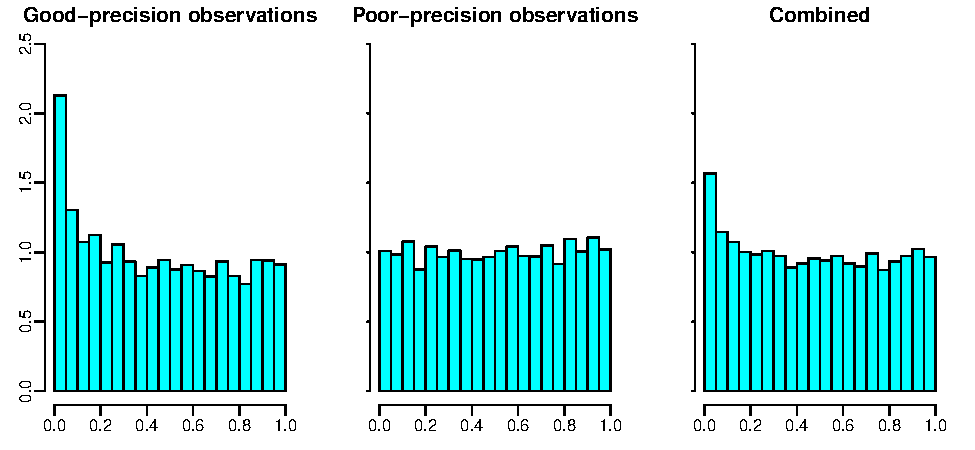
\includegraphics[width=4in]{../analysis/figure/make_GOODPOOR_figs.Rmd/GOODPOOReg_hist-1.pdf} 
    \label{fig:goodpoor-hist}
    \caption{Density histograms of $p$ values for good-precision, poor-precision, and combined observations}
 \end{subfigure}
\begin{subfigure}{\textwidth}
\centering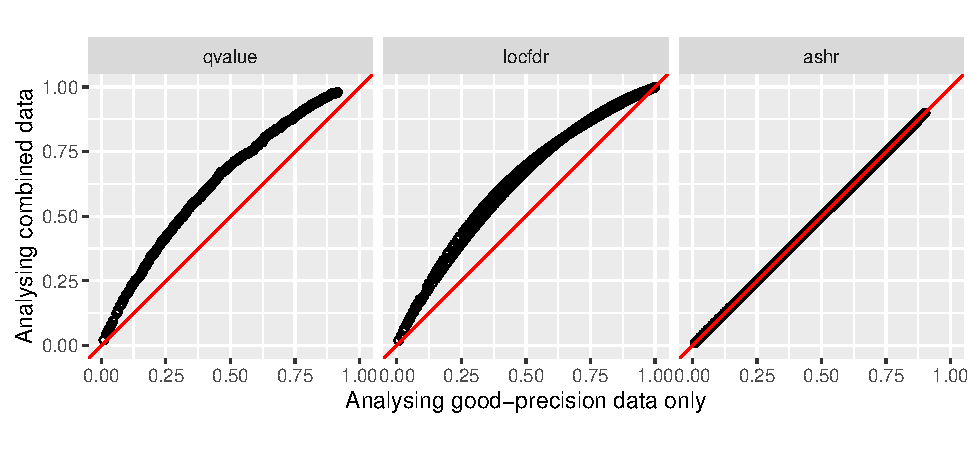
\includegraphics[width=4in]{../analysis/figure/make_GOODPOOR_figs.Rmd/GOODPOOReg_scatter-1.pdf}
    \caption{Comparison of results of different methods applied to good-precision observations only ($x$ axis) and combined data ($y$ axis). Each point shows the ``significance" ($q$ values from \qvalue; $\lfdr$ for \locfdr; $\lfsr$ for \ashr) of a good-precision observation under the two different analyses.} \label{fig:goodpoor-scatter}
\end{subfigure}
\caption{Simulation illustrating how, for existing FDR methods, 
poor-precision observations can contaminate signal from good-precision observations. The top panel (a) illustrates that when 
$p$ values from good-precision observations (left) and from poor-precision observations (center) are combined (right), they produce
a distribution of $p$ values with less overall signal - and so, by conventional methods, will give a higher estimated FDR at any given threshold.
The bottom panel (b) illustrates this behavior directly for the methods \qvalue and \locfdr: the $q$-values from \qvalue and the $\lfdr$ estimates from \locfdr are higher when applied to all data than when applied to good-precision observations only. In contrast the methods described here (\ashr) produce effectively the same results (here, the lfsr) in the good-precision and combined data analyses.} \label{fig:goodpoor}
\end{figure}


 \subsubsection*{Reordering of significance, and the ``$p$ value prior"}

Another consequence of accounting for differences in measurement precision is that \ashr may re-order the significance of the observations compared
 with the original $p$ values or $z$ scores. This is illustrated, using the same simulation as above, in Figure \ref{fig:lfsr_pval} (left panel).
 We see that poor precision measurements are assigned a higher $\lfsr$ than good precision measurements that have the same $p$ value.
 The intuition is that, due to their poor precision, these measurements contain very little information about the sign of the effects (or indeed any other aspect of the effects),
 and so the $\lfsr$ for these poor-precision measurements is always high.
 
The potential for Bayesian analyses to re-order the significance of observations, and specifically to down-weight imprecise observations,
was previously discussed in \cite{guan.stephens.08}. However, Wakefield \cite{wakefield:2009} showed that, under a certain prior assumption, the Bayesian analysis produces the same ranking of significance as $p$ values (or their $z$ scores). He named this prior the ``$p$-value prior" because it can be thought of as the 
implicit prior assumption that is being made if we rank the significance of observations by their $p$ value.
Wakefield's $p$-value prior assumes that the less precise effect estimates correspond to larger true effects, and specifically that they scale proportional
to the standard errors $s_j$. More specifically still, it assumes a normal prior for the non-zero $\beta_j$ with mean 0 and variance $K s^2_j$ for some constant $K$.
Here we observe that Wakefield's result extends to our mixture of (zero-mean) normal priors. Specifically, if, instead of assuming that $\beta_j$ is independent
of $s_j$ as we have up to now, we assume that $z_j=\beta_j/s_j$ is independent of $s_j$, and drawn from a mixture of zero-mean normal distributions,
then the $\lfsr$ computed by ash.n provides the {\it same ranking} of observations as the $z$ scores and $p$ values,
as is illustrated in Figure \ref{fig:lfsr_pval}, right panel. (This result does not hold when using the mixtures of uniforms prior, ash.u.)

This $p$-value prior assumes that the $z$ scores $z_j=\beta_j/s_j$
are identically distributed, independent of $s_j$. This is essentially the assumption made, implicitly or explicitly, by existing methods -- like \locfdr, \mixfdr and \qvalue --
that model the $z_j$ or $p_j$ directly.  In contrast, we have assumed up to now that the $\beta_j$ are independent of $s_j$. 
We can set both these assumptions within a more general framework, which allows that $\beta_j/s^\alpha$ is independent of $s_j$ for some $\alpha$ [Equation (\ref{eqn:beta-alpha}))]. Setting $\alpha=0$ implies that $\beta_j$ is
independent of $s_j$, as we have assumed up to now, and $\alpha>0$ implies that observations with larger standard error tend to have larger
effects (in absolute value). This latter assumption may often be qualitatively plausible: 
for example, in gene expression studies the standard error for gene $j$ depends partly on
the variance of its expression among samples, and genes with a larger variance may tend to be less tightly regulated and
so be amenable to a larger shift in expression between conditions (i.e.~larger effect $\beta_j$).
On the other hand, there is no particular reason to expect that either $\alpha=1$ or $\alpha=0$ will be the optimal choice.
Indeed, optimal choice of $\alpha$ will depend on the actual relationship between $\beta_j$ and $s_j$,
which will be dataset-specific. 
Framing the problem in this way -- that is, as comparing different modelling assumptions for $\beta_j$, rather than as 
comparing ``modelling $\beta_j$" vs  ``modelling $z_j$" (or ``modelling $p_j$") -- has the important advantage that 
likelihood-based methods can be used to select $\alpha$. For example, following the logic of the EB approach it
would be natural to select $\alpha$ by maximum likelihood. Since $\alpha$ is a one-dimensional parameter, this can be achieved by a 1-d grid search,
which has been implemented in our software by C. Dai. 

%\begin{result}
%If the prior distribution on $\beta/s | s$ is a mixture of zero-centered normal distributions, (\ref{eqn:mixnorm}), and the likelihood for $\beta$ is 
%given by $\bhat | s, \beta \sim N(0,s^2)$ then $p(\beta>0 | \bhat, s)$ is a monotonic increasing function of the $z$ score, $\bhat/s$. 
%\end{result}



%To summarize: the behaviour of \ashr depends on the value of $\alpha$ assumed in (\ref{eqn:beta-alpha}). 
%Up to now we have assumed $\alpha=0$, which implies that effects are identically distributed, independent of their standard error.
%In contrast, existing methods effectively assume $\alpha=1$, which implies that effects tend to scale proportional to their standard error.
%Whether it is better to set $\alpha=0$ or $\alpha=1$ in practice will depend on actual relationship between $\beta_j$ and $s_j$,
%which will be dataset-specific. Indeed, it seems quite likely that, in general, the optimal $\alpha$ may be some other (non-integer) value.
%(Alternatively, since fractional values of $\alpha$ may be tricky to interpret, users
%may prefer to simply choose whichever of $\alpha=0,1$ yields the highest likelihood.) 


%\begin{result}
%Treat the standard errors $s_j$ as fixed and given. Under the normal likelihood (\ref{eqn:normlik}), and using a mixture of normals for the prior distribution 
%(\ref{eqn:beta-alpha}) with $\alpha=1$, 
%the (Bayesian) $\lfsr_j$ and $\lfdr_j$ are all monotonic with $|t_j|$ where $t_j = \bhat_j/s_j$, and with the corresponding $p$ value $(p_j)$. Also, the shrinkage factor ($\text{Posterior Mean($\beta_j$)}/\bhat_j$) 
%is montonic with $|t_j|$. 
%\end{result}

 
%It is straightforward to prove, by performing Bayesian analysis for the standardized b$-J$
%Actually the key requirement is that the prior be such that the $t$ statistics $beta_j/s_j | s_j$ are identically distributed under the alternative.

%Most previous authors of EB approaches to false discovery rates \cite{efron2008microarrays,muralidharan2010empirical}
%have worked with models for $z$ scores $\beta_j/s_j$, rather than models for the effects $\beta_j$.
%In doing this they assume (implicitly or explicitly) that the $z$ scores are identically distributed under the alternative model.
%This is analogous
%to assuming $\alpha=1$ in (ref{eqn:beta-alpha}). And, given the result above, 
%standard frequentist FDR methods, like \qvalue and Benjamini--Hochberg, 
%that rank tests by their $p$ value, could also be viewed as making the same implicit assumption.



\begin{figure}
\centering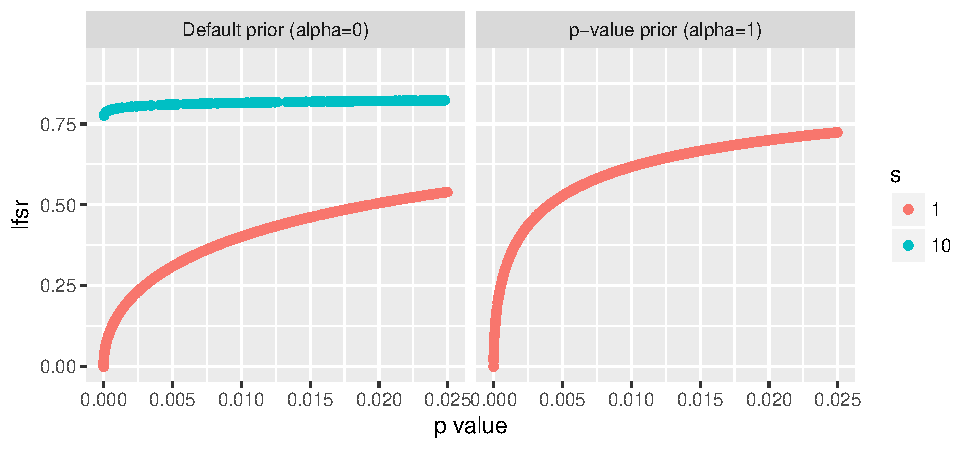
\includegraphics[width=4in]{../analysis/figure/make_GOODPOOR_figs.Rmd/lfsr_vs_pval_GOODPOOR-1.pdf}
\caption{Figure illustrating affects of prior assumptions on re-ordering of significance. Left panel shows results under our ``default prior" which assumes that effects $\beta_j$ are identically distributed, independent of $s_j$. Right panel shows results under the ``$p$-value prior", which assumes that $z$ scores $\beta_j/s_j$ are identically distributed, independent of $s_j$.} \label{fig:lfsr_pval}
\end{figure}

%\subsubsection*{Adaptive Shrinkage}
%
%Johnstone and Silverman \cite{johnstone2004needles} (see also \cite{raykar2011empirical}) note the ability of EB methods to adapt to overall signal strength
%when attempting to identify and estimate strong signals. The idea is that, if most $\beta_j$ are truly at or near zero then (given enough data) 
%the estimated prior distribution $\hat{g}$ will reflect this by being concentrated near 0, and the posterior distributions
% $p(\beta_j | \bhat_j, \shat_j,\hat{g})$ will consequently also tend to concentrate around zero (strong shrinkage). 
% In contrast, if most $\beta_j$ are large then $\hat{g}$ will be flatter, resulting in less shrinkage.
% Indeed, in the limit as $\hat{g}$ becomes flatter and flatter the posterior distribution on $\beta_j$ becomes $N(\bhat_j,\shat_j)$,
% and the Bayesian credible intervals match standard confidence intervals, which might be considered ``no shrinkage".
%
%Our methods we build on this idea in two ways. First,
%by using flexible semi-parametric approaches to estimate $g$ we aim to maximise the potential for this adaptive behaviour.
%Second, by incorporating the precision of each measurement into the likelihood, (\ref{eqn:normlik}) or (\ref{eqn:tlik}), we ensure that shrinkage
%adapts to measurement precision: more precise measurements undergo
% less shrinkage than less precise measurements.  This is because observations $\bhat_j$ with larger standard errors have flatter likelihoods 
%than observations with
%small standard error, and so their posteriors will be more affected by the prior, which, being unimodal at 0, tends to shrink estimates towards 0. 
%To emphasize these two key features we refer to our method as ``{\bf a}daptive {\bf sh}rinkage".
%Figure \ref{fig:ash} illustrates the idea by contrasting results for two simulation scenarios with different signal strengths, where observations vary in their measurment precision.
%
%\begin{figure}[!ht]
%\begin{center}
%\includegraphics[width=400px]{../examples/ash.pdf} 
%\end{center}
%\caption{Figure illustrating adaptive shrinkage. Results are shown for two different scenarios: (left) ``big-normal" where the effects have a wide distribution; (right) ``spiky", where the effects are more concentrated near 0. The standard error of each observation, $s_j$, was simulated from Inverse Gamma(5,5), which resulted in $s_j$ varying from 0.34 to 6.7.  The shrunken estimates ($y$ axis) are plotted against the observed estimates ($x$ axis), with color indicating the (square root of the) precision of each measurement (blue=lower-precision; red=higher-precision). The two key features are i) shrinkage is adaptive to signal in data, so shrinkage is stronger for the spiky scenario; ii) shrinkage is adaptive to the precision of each measurement, so less precise observations (blue) are shrunken more strongly.} \label{fig:ash}
%\end{figure}

%DISCUSSION ON ADAPTIVE SHRINKAGE; BEST TO PUT IN RESULTS?
%To understand how this approach leads to ``adaptive shrinkage", think of (\ref{eqn:betaj}) as defining the ``prior distribution" for $\beta_j$ (determined by hyper-parameters $\pi$),  and (\ref{eqn:bhat}) as defining the likelihood for $\beta_j$. Because the prior distribution is unimodal about zero, 
%the posterior distribution of $\beta$ will be ``shrunk" towards zero (compared with the likelihood), with the
%amount of shrinkage being determined by a) how concentrated the prior is near zero (determined by $\hat{\pi}$) and b) how concentrated the likelihood is around $\bhat_j$.
%For example, if most $\beta_j$ are truly at or near zero then $\hat\pi$ will concentrate on zero and very small values of $\sigma_k$, and this will produce stronger shrinkage
%than if $\beta_j$ are mostly large. And observations $\bhat_j$ with large standard error will have flatter likelihoods than observations with
%small standard error, and so their posteriors will be more affected by the prior, and undergo more shrinkage. 

%previous work based on normal means:
%http://link.springer.com/article/10.1007/BF02562623


%\subsection{Null behaviour}

%Results of simulations under the null.

%\subsection{Comparison of different underlying component distributions}
%
%Because the mixture of zero-anchored uniforms is more flexible than the mixture of zero-centered uniforms, which is more flexible
%than the mixture of zero-centered normals, we expect that the likelihoods will satisfy $L_{hu} > L_u > L_n$. However, for Scenario A we expect the differences in
%likelihood to be small, because the true model here is a mixture of zero-centered normals, so any gain of $L_{hu}$ and $L_u$ over $L_n$ is necessarily due to ``overfitting".
%For Scenario B, we expect that $L_{hu}$ and $L_{u}$ to be significantly larger than $L_n$, but any 
%increase of $L_{hu}$ over $L_u$ must be due to overfitting (because the truth is symmetric). Finally, for Scenario C we
%expect $L_{hu}$ to be significantly larger than the others.
%
%Figure \ref{fig:rmse_loglik_boxplot} illustrates this.
%
%\begin{figure}[!ht] \label{fig:rmse_loglik_boxplot}
%\begin{center}
%\includegraphics[width=6.5in]{Rcode/figures/simABC_egdens.pdf}
%%\includegraphics[width=6.5in]{Rcode/figures/rmse_loglik_boxplot.pdf}
%\includegraphics[width=6.5in]{Rcode/figures/rmse_boxplot.pdf}
%\includegraphics[width=6.5in]{Rcode/figures/loglik_boxplot.pdf}
%\end{center}
%\caption{}
%\end{figure}

%Notes from Adrian Raftery - 
%Newcombe (1886)
%Dean and Raftery
%Uniform is super-efficient

\section*{Discussion}

We have presented an Empirical Bayes approach to large-scale multiple testing that emphasizes two ideas.
First, we emphasize the potential benefits of using two numbers ($\bhat$, and its standard error)
rather than just one number (a $p$ value or $z$ score)  to summarize the information on each test.
While requiring two numbers is slightly more onorous than requiring one, in many settings these
numbers are easily available and if so we argue it makes sense to use them.
Second, we note the potential benefits -- both statistical and computational -- of assuming that the effects come from a unimodal distribution, and provide
flexible implementations for performing inference under this assumption. We also introduce the ``false sign rate" as
an alternative measure of error to the FDR, and illustrate its improved robustness to errors in model fit, particularly mis-estimation
of the proportion of null tests, $\pi_0$.

Multiple testing is often referred to as a ``problem" or a ``burden". In our opinion, EB approaches turn this idea on its head,
treating multiple testing as an {\it opportunity}: specifically, an opportunity to learn about the prior distributions, and other modelling assumptions,
to improve inference and make informed decisions about significance (see also \cite{greenland1991empirical}). This view
also emphasizes that, what matters in multiple testing settings is {\it not} the number of tests, but the {\it results} of the tests.
Indeed, the FDR at a given fixed threshold does not depend on the number of tests: as the number of tests increases, both the true positives and false positives increase linearly,
and the FDR remains the same. (If this intuitive argument does not convince, see \cite{storey.03}, and note that the FDR at a given $p$ value threshold does not depend on the number of tests $m$.) Conversely, the FDR {\it does} depend on the overall distribution of effects, and particularly on $\pi_0$ for example. 
The EB approach captures this dependence in an intuitive way:
if there are lots of strong signals then we infer $\pi_0$ to be small, and the estimated FDR (or $\lfdr$, or $\lfsr$) at a given threshold may be low, even if a large number of tests were performed; and conversely
if there are no strong signals then we infer $\pi_0$ to be large and the FDR at the same threshold may be high, even if relatively few tests were performed. 
More generally, overall signal strength is reflected in the estimated $g$, which in turn influences the estimated FDR.

Two important practical issues that we have not addressed here are correlations among tests,
and the potential for deviations from the theoretical null distributions of test statistics. These two
issues are connected: specifically, unmeasured confounding factors can cause both correlations among tests
and deviations from the theoretical null \cite{efron2007correlation,leek:2007}. And although there are certainly other
factors that could cause dependence among tests, unmeasured confounders are perhaps the most worrisome in practice
because they can induce strong correlations among large numbers of tests and profoundly impact results, ultimately resulting
in too many hypotheses being rejected and a failure to control FDR.
We are acutely aware that, because our method is less conservative than existing methods, it may unwittingly
exacerbate these issues if they are not adequately dealt with.
Approaches to deal with unmeasured confounders can be largely divided into two types: those
that simply attempt to correct for the resulting inflation of test statistics \cite{devlin1999genomic,efron2004large}, and those
that attempt to infer confounders using clustering, principal components analysis, or factor models 
\cite{pritchard.stephens.rosenberg.donnelly.00,price:2006,leek:2007,gagnon2012using},
and then correct for them in computation of the test statistics (in our case, $\bhat,\shat$). When these latter approaches are viable
they provide perhaps the most satisfactory solution, and are certainly a good fit for our framework. Alternatively, our methods
could be modified to allow for test statistic inflation, an idea that may be worth pursuing in future work.


Another important practical issue is the challenge of small sample sizes. For example, in genomics applications researchers sometimes
attempt to identify differences between two conditions based on only a handful of samples in each. In such settings the
normal likelihood approximation (\ref{eqn:normlik}) will be inadequate. And, although the $t$ likelihood (\ref{eqn:tlik}) partially
addresses this issue, it is also, it turns out, not entirely satisfactory.  The root of the problem is that, with small sample sizes, raw estimated standard
errors $\shat_j$ can be horribly variable. In genomics it is routine to address this issue by applying EB methods \cite{smyth:2004} to ``moderate" (i.e.~shrink) variance estimates,
before computing $p$ values from ``moderated" test statistics. We are currently investigating how
our methods should incorporate such ``moderated" variance estimates to make it applicable to small sample settings.

Our approach involves compromises between flexibility, generality, and simplicity on the one hand, and statistical efficiency and principle on the other.
For example, in using an EB approach that uses a point estimate for $g$, rather than a fully Bayes approach that accounts for uncertainty in $g$,
we have opted for simplicity over statistical principle. And in summarizing every test by
two numbers and making a normal or $t$ approximation to the likelihood, we have aimed to produce generic methods that 
 can be applied whenever such summary data are available -- just as \qvalue can be applied to any set of $p$ values for example -- although
 possibly at the expense of statistical efficiency compared with developing multiple tailored approaches based on context-specific likelihoods. 
 Any attempt to produce generic methods will involve compromise between generality and efficiency.
 In genomics, many analyses -- not only FDR-based analyses -- involve first computing a series of $p$ values before
 subjecting them to some further downstream analysis. An important message here is 
 that working with two numbers ($\bhat_j,\shat_j$), rather than one ($p_j$ or $z_j$), 
 can yield substantial gains in functionality (e.g.~ estimating effect sizes, as well as testing; accounting for variations in
measurement precision across units) while losing only a little in generality.  We hope that our work will
encourage development of methods that exploit this idea in other contexts.

%This is connected with work by \cite{wakefield:2009} (see also \cite{johnson:2008}) who performs Bayesian inference
%from summary statistics, computing $p(\beta_j | \bhat_j, \shat_j)$ for a single $j$,
%with a specific fixed prior on $\beta_j$. Essentially we extend this to multiple $j$, using a hierarchical model to connect the observations.
 



%
%
%Both \locfdr and \mixfdr allow for deviations from
%the theoretical null distribution by allowing that, under the null, the $z$ scores are $N(0,\sigma^2)$ with $\sigma$ estimated from the data rather
%than fixed to 1. Within our approach this idea could be incorporated by changing the likelihood - for example, to assume $\bhat_j \sim N(0,s_ 
%
%These are tricky issues that, as far as we are aware, can affect
%all approaches to FDR analysis. An important focus of Efron's work, also implemented in \locfdr, 
% is to relax the assumption that the null $z$ scores are $N(0,1)$, to allow for empirical deviations from this
%theoretical null distribution. 
%
%For example, we and others have worked on Bayesian approaches to genetic association testing, using subjective prior specification of
%effect sizes based on external data (e.g.~\cite{stephens:2009}). However, the large numbers of tests brings the opportunity to learn about
%priors, and here we aim to exploit this 

%Choice of mixture components. Use of likelihood to compare different mixture components?



%  
%Directly modeling the p values, or z scores, say via non-parametric methods, 
%can lead to unrealistic distributions being fitted. Put another way, because z scores are the result of adding noise to some
%distribution, the range of distributions they can take is limited Using entirely non-parametric methods loses this information.
%The solution is to model beta hat as a convolution of some distribution g and an error component.


%Before proceeding, we feel obliged to correct the common misconception
% that the use of FDR methods is to ``correct" for the number of tests performed. In fact the FDR does
% not depend on the number of tests. 
%  A better way to think of it is that the FDR accounts for the {\it amount of signal} in the tests that were performed: 
% 
% In other words, FDR corrects for the {\it results} of all tests performed, not the {\it number} of all tests performed.
 
 







\section*{Detailed Methods} \label{sec:implement}

\subsection*{Embellishments} 

\subsubsection*{More flexible unimodal distributions}

Using a mixture of zero-centered normal distributions for $g$ in (\ref{eqn:mixnorm}) implies that $g$ is not only unimodal, but also symmetric.
Furthermore, even some symmetric unimodal distributions, such as those with a flat top, cannot be well approximated by a mixture of zero-centered normals.
 Therefore, we have implemented a more general approach based on 
\begin{equation} \label{eqn:g-general}
g(\cdot; \pi) = \sum_{k=0}^K \pi_k f_k(\cdot) ,
\end{equation}
where $f_0$ is a point mass on 0, and $f_k$ ($k=1,\dots,K$) are pre-specified component distributions with one of the following forms: 
\begin{enumerate}[(i)]
\item $f_k(\cdot) = N(\cdot; 0, \sigma^2_k)$, \qquad (``ash.n")
\item $f_k(\cdot) = U[\cdot; -a_k,a_k]$,  \qquad (``ash.u")
\item $f_k(\cdot) = U[\cdot; -a_k,0] \text{ and/or } U[\cdot; 0,a_k]$,  \qquad (``ash.hu")
\end{enumerate}
where $U[\cdot; a,b]$ denotes the density of a uniform distribution on $[a,b]$.
(In (iii) we include both components in the mixture (\ref{eqn:g-general}), so a grid of values $a_1,\dots,a_K$ defines $2K+1$ mixture component densities, 
and $\pi$ is a $2K+1$ vector that sums to 1.)
The simplest version (\ref{eqn:mixnorm}) corresponds to (i).
Replacing these with uniform components (ii)-(iii) only slightly complicates calculations
under the normal likelihood (\ref{eqn:normlik}), and greatly simplifies the calculations under the $t$ likelihood
(\ref{eqn:tlik}) introduced below. The use of uniform components here closely mirrors \cite{cordy1997deconvolution}.
(In fact our implementation can handle {\it any} pre-specified uniform or normal distributions for $f_k$ provided they are all from the same family;
however, we restrict our attention here to (i)-(iii) which imply a unimodal $g$.)

Moving from (i) to (iii) the representation (\ref{eqn:g-general}) becomes increasingly flexible. Indeed,
using a large dense grid of $\sigma^2_k$ or $a_k$, (i)-(iii) can respectively approximate,
with arbitrary accuracy,
\begin{enumerate}[(i)]
\item any scale mixture of normals, which includes as special cases
the double exponential (Laplace) distribution, any $t$ distribution, and a very large number of other distributions used in  high-dimensional regression settings.
\item any symmetric unimodal distribution about 0.
\item any unimodal distribution about 0.
\end{enumerate}
The latter two claims are related to characterizations of unimodal distributions due to \cite{khintchine1938unimodal} and  \cite{shepp1962symmetric}; see \cite{feller1971introduction}, p158. 
In other words, (ii) and (iii) provide fully non-parametric estimation for $g$ under the constraints that it is (ii) both unimodal and symmetric, or (iii) unimodal only.

Although our discussion above emphasizes the use of large $K$, in practice modest values of $K$ can provide reasonable performance. 
The key point is that the value of $K$ is not critical provided it is sufficiently large, and the grid of $\sigma_k$ or $a_k$ values suitably chosen.
See Implementation for details of our software defaults.

%Although it is natural to worry about ``overfitting" if $K$ is large,  in fact the unimodal constraint is sufficient to prevent serious problems with overfitting. For example, note that the unimodal constraint is sufficiently strong that there will exist a non-parametric maximum likelihood estimate (NPMLE) for $g$ under this constraint. (Indeed, if the $\beta_j$ are observed without error, corresponding to the standard errors $\shat_j \rightarrow 0$, this NPMLE has an explicit and elegant form; \cite{grenander1956theory}.)
%Thus allowing $K$ to be large in ii) or iii), and maximizing the likelihood with respect to $\pi$, will approximate the NPMLE for $g$, under the constraints of symmetry and unimodality (ii), or unimodality alone (iii). 

\subsubsection*{Dependence of effects on standard errors}

Equation (\ref{eqn:beta}) assumes that the $\beta_j$ all come from the same distribution $g$, independent of $\shat_j$.
This can be relaxed to allow the distribution of $\beta_j$ to depend on $\shat_j$ using
 \begin{equation} \label{eqn:beta-alpha}
 \frac{\beta_j}{\shat_j^\alpha} \, \big |  \shat_j \sim g(\cdot; \pi)
 \end{equation}
for any $\alpha$. Setting $\alpha=0$ yields (\ref{eqn:beta}), and setting $\alpha=1$ corresponds to
assuming that the $t_j =\beta_j/ \shat_j$ have a common distribution. This case is of special interest:
it effectively corresponds to the ``$p$ value prior" in \cite{wakefield:2009} and is, implicitly, 
the assumption made by existing FDR methods that rank tests by their $p$ values (or $z$ or $t$ scores). See Results for further discussion.
 
The model \ref{eqn:beta-alpha} for general $\alpha$ can be fitted using the algorithm for $\alpha=0$. 
To see this, define $b_j:= \beta_j/ \shat_j^\alpha$, and $\hat{b} := \bhat_j/\shat_j^\alpha$. Then $\hat{b}_j$ is an estimate of $b_j$ with
 standard error $\shat'_j:=\shat_j^{1-\alpha}$. 
 Applying the algorithm for $\alpha=0$ to effect estimates $\hat{b}_1,\dots,\hat{b}_J$ with standard errors $\shat'_1,\dots,\shat'_J$
yields a posterior distribution $p(b_j | \shat_j, \hat{b}_j, \hat{\pi}, \alpha)$, which induces a posterior distribution on $\beta_j = b_j \shat_j^\alpha$.
%In the special case $\alpha=1$, $\hat{b}_j$ is the $t$ score $t_j$ and $\shat'{b}=1$, so this involves applying our algorithm to the $t$ scores
%treating them all as having the same standard error. In this case the local fdr from our method becomes monotonic in each direction as
%the $t$ score increases away from zero, just as with \qvalue, and (usually) \mixfdr and \locfdr.

%Different values of $\alpha$ in (\ref{eqn:beta-alpha}) essentially correspond to different models for
%how effect sizes $\beta_j$ scale with the standard error $\shat_j$. Since this scaling is unknown it may be desirable to estimate
%it from the data, and this can be done here by jointly maximizing the likelihood $p(\hat{b} | \shat,\pi,\alpha)$ over $\pi$ and $\alpha$
%rather than just $\pi$.  Although values of $\alpha$ other than 0 and 1 may not be easy interpret,
%and the actual relationship between $\beta_j$ and $\shat_j$ is unlikely to exactly follow (\ref{eqn:beta-alpha}) for any $\alpha$,
%this approach seems preferable in practice than simply assuming $\alpha=0$ or $\alpha=1$. We
%do not investigate this in detail here, but it has been implemented in our software by C.Dai, using a simple grid search over $\alpha$.


\subsubsection*{Replace normal likelihood with $t$ likelihood}

We generalize the normal likelihood (\ref{eqn:normlik}) by replacing it with a $t$ likelihood:
  \begin{equation} \label{eqn:tlik}
 \bhat_j \, | \, \beta_j, \shat_j \sim T_\nu(\beta_j, \shat_j)
 \end{equation}
where $T_\nu(\beta_j,\shat_j)$ denotes the distribution of $\beta_j+\shat_j T_\nu$ where $T_\nu$ has a standard $t$ distribution on $\nu$ degrees of freedom,
and  $\nu$ denotes the degrees of freedom used to estimate $\shat_j$ (assumed known, and for simplicity assumed to be the same for each $j$).
The normal approximation (\ref{eqn:normlik}) corresponds to the limit $\nu \rightarrow \infty$.
This generalization does not complicate inference when the mixture components $f_k$ in (\ref{eqn:g-general}) are uniforms; see Implementation below.
When the $f_k$ are normal the computations with a $t$ likelihood are considerably more difficult and we have not implemented this combination.

Equation (\ref{eqn:tlik}) is, of course, motivated by the standard asymptotic result
\begin{equation} \label{eqn:tdist}
(\bhat_j-\beta_j)/\shat_j \sim T_\nu.
\end{equation}
However (\ref{eqn:tdist}) does not imply (\ref{eqn:tlik}), because in (\ref{eqn:tdist}) $\shat_j$ is random whereas in (\ref{eqn:tlik}) it is conditioned on.
In principle it would be preferable, for a number of reasons, to model the randomness in $\shat_j$; we are
currently pursuing this improved approach (joint work with M.Lu) and results will be published elsewhere. 
%We note here that
%modelling the randomness in $\shat_j$ is particularly helpful when the number of observations used to estimate $\shat_j$ is very small (e.g. $<10$),
%where our simpler approach can produce unsatisfactory results.

\subsubsection*{Non-zero mode}

An addition to our software implementation, due to C.Dai, allows the mode to be estimated from the data by maximum likelihood, rather than fixed to 0.
This involves a simple grid search. 

\subsection*{Implementation Details}

\subsubsection*{Likelihood for $\pi$}

We define the likelihood for $\pi$ to be the probability of the observed data $\bhat$ conditional on $\shat$: $L(\pi) := p(\bhat | \shat,\pi),$ which
by our conditional independence assumptions is equal to the product $\prod_j p(\bhat_j | \shat, \pi)$. [One might prefer to define the likelihood as $p(\bhat, \shat | \pi) = p(\bhat | \shat, \pi) p(\shat | \pi)$, in which case our definition comes down to assuming that the term $p(\shat | \pi)$ does not depend on $\pi$.]

Using the prior $\beta_j \sim \sum_{k=0}^K \pi_k f_k(\beta_j)$ given by (\ref{eqn:g-general}), and the normal likelihood (\ref{eqn:normlik}), integrating over $\beta_j$ yields
\begin{equation}
p(\bhat_j | \shat,\pi)  = \sum_{k=0}^K \pi_k \tilde{f}_k(\bhat_j)
\end{equation}
where 
\begin{equation}
\tilde{f}_k(\bhat_j) := \int f_k(\beta_j) N(\bhat_j; \beta_j,\shat^2_j) \, d\beta_j
\end{equation}
denotes the convolution of $f_k$ with a normal density.
These convolutions are straightforward to evaluate whether $f_k$ is a normal or uniform density.
Specifically, 
\begin{equation} \label{eqn:uconv}
\tilde{f}_k(\bhat_j)  = 
\begin{cases}
N(\bhat_j;0, \shat_j^2 +  \sigma_k^2) & \text{if $f_k(\cdot) = N(\cdot; 0, \sigma_k^2)$}, \\
\frac{\Psi((\bhat_j-a_k)/\shat_j) - \Psi((\bhat_j-b_k)/\shat_j)}{b_k-a_k} & \text{if $f_k(\cdot) = U(\cdot; a_k,b_k)$},
\end{cases}
\end{equation}
where $\Psi$ denotes the cumulative distribution function (c.d.f.) of the standard normal distribution.
If we replace the normal likelihood with the $t_\nu$ likelihood (\ref{eqn:tlik}) then the convolution 
for $f_k$ uniform the convolution is still given by (\ref{eqn:uconv}) but with $\Psi$ the c.d.f. 
of the $t_\nu$ distribution function. (The convolution for $f_k$ normal is tricky and we have not implemented it.)

\subsubsection*{Penalty term on $\pi$}

To make $\lfdr$ and $\lfsr$ estimates from our method ``conservative" we add a penalty 
term $log(h(\pi;\lambda))$ to the log-likelihood $\log L(\pi)$ to encourage over-estimation of $\pi_0$:
\begin{equation} \label{eqn:penalty}
h(\pi;\lambda) = \prod_{k=0}^K \pi_k^{\lambda_k-1}
\end{equation}
where $\lambda_k \geq 1 \, \forall k$. The default is $\lambda_0=10$ and $\lambda_k=1$, which yielded
consistently conservative estimation of $\pi_0$ in our simulations (Figure \ref{fig:pi0sims}). 

Although this penalty is based on a Dirichlet density, we do not interpret this as a ``prior distribution" for $\pi$:
we chose it to provide conservative estimates of $\pi_0$ rather than to represent prior belief.

\subsubsection*{Problems with removing the penalty term in the half-uniform case}

It is straightforward to remove the penalty term by setting $\lambda_k=1$ in (\ref{eqn:penalty}).
We note here an unanticipated problem we came across when using no penalty term in the half-uniform case 
(i.e.~ $f_k(\cdot) = U[\cdot; -a_k,0] \text{ and/or } U[\cdot; 0,a_k]$ in (\ref{eqn:g-general})): when the data
are nearly null, the estimated $g$ converges, as expected and desired, to a distribution where almost all the mass is near 0, but
sometimes all this mass is concentrated almost entirely just to one side (left or right) or 0. This can have a very profound effect on the local false sign rate:
for example, if all the mass is just to the right of 0 then all observations will be assigned a very high probability of being positive (but very small),
and a (misleading) low local false sign rate. For this reason we do not recommend use of the half-uniform with no penalty.


\subsubsection*{Optimization}

With this in place, the penalized log-likelihood for $\pi$ is given by:
\begin{equation}
\log L(\pi) + \log h(\pi) = \sum_{j=1}^n \log(\sum_{k=0}^K \pi_k l_{kj}) + \sum_{k=0}^K (\lambda_k-1) \log \pi_k
\end{equation}
where the $l_{kj}:= \tilde{f}_k(\bhat_j)$ are known. This is a convex optimization problem, which
can be solved very quickly and reliably using interior point (IP) methods. We used the {\tt KWdual} function from the {\tt R} package {\tt REBayes} \cite{REBayes}, which uses {\tt Rmosek} \cite{Rmosek}. We also found a simple EM algorithm \cite{dempster77}, accelerated using the elegant {\tt R} package {\tt SQUAREM} \cite{varadhan2008simple},
to provide adequate performance. In our EM implementation we initialized $\pi_k=1/n$ for $k=1,\dots,K$, with $\pi_0=1-\pi_1-\dots-\pi_K$,
and the one-step updates are:
\begin{align} \label{eqn:w}
w_{kj} & = \pi_k l_{kj} / \sum_{k'} {\pi_{k'} l_{k'j}} \\
n_k & = \sum_j w_{kj} + \lambda_k - 1 \quad \text{[E Step]} \\
\pi_k &= n_k/\sum_{k'} n_{k'} \quad \text{[M step]}.
\end{align}
One benefit to the EM algorithm is fewer software dependencies.
Both EM and IP methods are implemented in the {\tt ashr} package; results shown here are from the IP method, but graphs from EM are essentially the same.
See \href{http://stephenslab.github.io/ash/analysis/checkIP.html}{http://stephenslab.github.io/ash/analysis/checkIP.html}  and \href{http://stephenslab.github.io/ash/analysis/IPvsEM.html}{http://stephenslab.github.io/ash/analysis/checkIP.html}  for comparisons.

\subsubsection*{Conditional distributions}

Given $\hat\pi$, we compute the conditional distributions 
\begin{equation}
p(\beta_j | \hat\pi, \bhat, s) \propto g(\beta_j; \pi) L(\beta_j; \bhat_j, \shat_j).
\end{equation} 
Each posterior is a mixture on $K+1$ components:
\begin{equation}
p(\beta_j | \hat\pi, \bhat, s) = \sum_{k=0}^K w_{kj} p_k(\beta_j | \bhat_j, \shat_j)
\end{equation}
where the posterior weights $w_{kj}$ are computed as in (\ref{eqn:w}) with $\pi=\hat\pi$,
and the posterior mixture component $p_k$ is the posterior on $\beta_j$ that would be obtained using prior 
$f_k(\beta_j)$ and likelihood $L(\beta_j; \bhat_j,\shat_j)$.
All these posterior distributions are easily available.
For example, if $f_k$ is uniform and $L$ is $t_\nu$ then this is a truncated $t$ distribution.
If $f_k$ is normal and $L$ is normal, then this is a normal distribution.



\subsubsection*{Choice of grid for $\sigma_k, a_k$} \label{sec:grid}

\def\sigmamax{\sigma_{\text{max}}}
\def\sigmamin{\sigma_{\text{min}}}
When $f_k$ is $N(0,\sigma_k)$ we specify our grid by specifying: i) a maximum and minimum value $(\sigmamin,\sigmamax)$; ii) a multiplicative factor $m$ to be used
in going from one grid-point to the other, so that $\sigma_{k} = m \sigma_{k-1}$. The multiplicative factor affects the density of the grid; we used $m=\sqrt{2}$
as a default. We chose $\sigmamin$ to be small compared with the measurement precision ($\sigmamin=\min(\shat_j)/10$) and $\sigmamax= 2\sqrt{\max(\bhat_j^2-\shat_j^2)}$
based on the idea that $\sigmamax$ should be big enough so that  $\sigmamax^2 + \shat_j^2$ should exceed $\bhat_j^2$.   (In rare cases where $\max(\bhat_j^2-\shat_j^2)$
is negative we set $\sigmamax = 8\sigmamin$.)

When the mixture components $f_k$ are uniform, we use the same grid for the parameters $a_k$ as for $\sigma_k$ described above.

Our goal in specifying a grid was to make the limits sufficiently large and small, and the grid sufficiently dense, that results would not change appreciably with 
a larger or denser grid. For a specific data set one can of course check this by experimenting with the grid, but these defaults usually work well in our experience.


\appendix

\begin{figure}
\begin{center}
\begin{subfigure}{\textwidth}
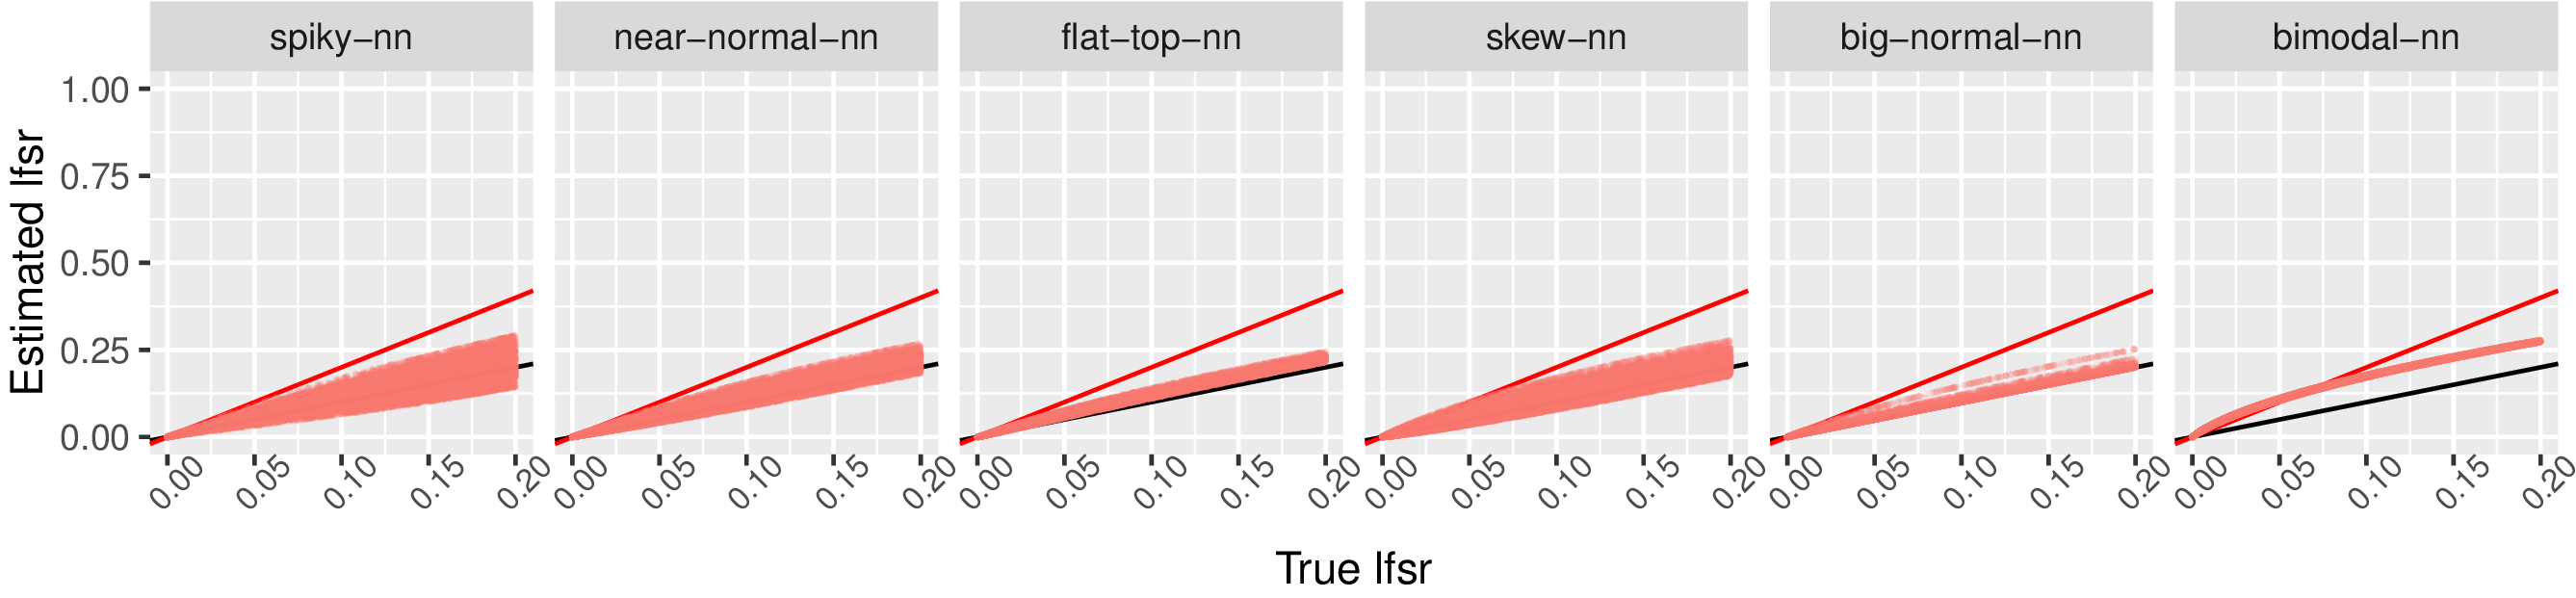
\includegraphics[width=\textwidth]{../analysis/figure/plot_lfsr.Rmd/plot_lfsr_s_nn-1.pdf} 
\caption{Comparison of true and estimated $\lfsr$ when data are simulated with no point mass at zero ($\pi_0=0$), and also analyzed by \ashr with no point mass on 0 (and mixture of normal components for $g$). Black line is $y=x$ and red line is $y=2x$. The results illustrate how estimates of $\lfsr$ can be more accurate in this case. That is, assuming there is no point mass can be beneficial if that is indeed true.}  \label{fig:lfsr-nn}
\end{subfigure}
\begin{subfigure}{\textwidth}
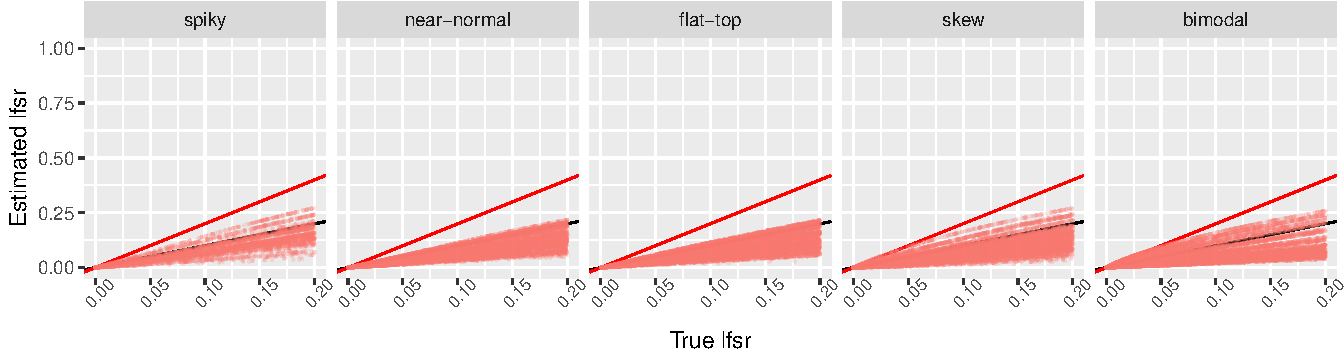
\includegraphics[width=\textwidth]{../analysis/figure/plot_lfsr.Rmd/plot_lfsr_s-1.pdf} 
\caption{Comparison of true and estimated $\lfsr$ when data are simulated with point mass at zero (drawn uniformly from [0,1] in each simulation), but analyzed by \ashr with no point mass on 0 (and mixture of normal components for $g$). Black line is $y=x$ and red line is $y=2x$. The results illustrate how estimates of $\lfsr$ can be anti-conservative if we assume there is no point mass when the truth is that there is a point mass.} \label{fig:lfsr-s}
\end{subfigure}
\end{center}
\caption{Illustration of effects of excluding a point mass from the analysis.} \label{fig:lfsr-nopointmass}
\end{figure}



\begin{table}[!ht]
\centering\begin{tabular}{c c } \toprule
Scenario & Alternative distribution, $g_1$  \\ \midrule
spiky & $0.4 N(0,0.25^2) + 0.2 N(0,0.5^2) + 0.2 N(0,1^2), 0.2 N(0,2^2) $\\
near normal & $2/3 N(0,1^2) + 1/3 N(0,2^2)$ \\
flattop& $(1/7) [N(-1.5,.5^2) + N(-1,.5^2) + N(-.5,.5^2) +$ \\
 &  $N(0,.5^2) +N(0.5,.5^2)  +N(1.0,.5^2) + N(1.5,.5^2)]$  \\
skew & $(1/4) N(-2,2^2) + (1/4) N(-1,1.5^2) +  (1/3) N(0,1^2) + (1/6) N(1,1^2) $\\
big-normal & $N(0,4^2)$ \\ 
bimodal & $0.5 N(-2,1^2) + 0.5 N(2,1^2)$ \\ \bottomrule
\end{tabular}
\caption{Summary of simulation scenarios considered} \label{table:scenarios}
\end{table}


\begin{table}[!ht]
\begin{subtable}{\textwidth}
	\centering% latex table generated in R 3.2.3 by xtable 1.7-4 package
% Sun Jan 24 15:11:56 2016
\begin{tabular}{rrrrrrr}
  \toprule  & spiky & near-normal & flat-top & skew & big-normal & bimodal \\ 
  \midrule ash.n.s & 0.95 & 0.95 & 0.95 & 0.95 & 0.96 & 0.96 \\ 
  ash.u.s & 0.94 & 0.95 & 0.95 & 0.94 & 0.96 & 0.96 \\ 
  ash.hu.s & 0.88 & 0.92 & 0.92 & 0.92 & 0.93 & 0.93 \\ 
   \bottomrule \end{tabular}


	\caption{All observations}
\end{subtable}

\begin{subtable}{\textwidth}
\centering% latex table generated in R 3.2.3 by xtable 1.7-4 package
% Sun Jan 24 15:11:55 2016
\begin{tabular}{rrrrrrr}
  \toprule  & spiky & near-normal & flat-top & skew & big-normal & bimodal \\ 
  \midrule ash.n.s & 0.95 & 0.95 & 0.98 & 0.93 & 0.95 & 0.97 \\ 
  ash.u.s & 0.89 & 0.92 & 0.90 & 0.92 & 0.94 & 0.94 \\ 
  ash.hu.s & 0.89 & 0.92 & 0.91 & 0.94 & 0.95 & 0.94 \\ 
   \bottomrule \end{tabular}


\caption{``Significant" negative discoveries.}
\end{subtable}

\begin{subtable}{\textwidth}
\centering% latex table generated in R 3.2.3 by xtable 1.7-4 package
% Tue Dec 15 18:12:54 2015
\begin{tabular}{rrrrrrr}
  \toprule  & spiky & near-normal & flat-top & skew & big-normal & bimodal \\ 
  \midrule ash.n.s & 0.94 & 0.94 & 0.92 & 0.88 & 0.95 & 0.94 \\ 
  ash.u.s & 0.93 & 0.93 & 0.92 & 0.88 & 0.95 & 0.95 \\ 
  ash.hu.s & 0.34 & 0.60 & 0.52 & 0.54 & 0.79 & 0.82 \\ 
   \bottomrule \end{tabular}


\caption{``Significant" positive discoveries.}
\end{subtable}

\caption{Table of empirical coverage for nominal 95\% lower credible bounds for methods {\it without} the penalty term). } \label{tab:nopen}
\end{table}
%In simple settings (e.g. symmetric effects, with the same standard error) $\fdr_j$ is a monotonic function of the $p$ value $p_j$, and so
%\begin{equation}
%q_j = \widehat\FDR(\{k:p_k \leq p_j\})
%\end{equation}
%which is close to the definition in \cite{storey.03}.


% Do NOT remove this, even if you are not including acknowledgments
\section*{Acknowledgements}

I thank J.~Lafferty for pointing out the convexity of the likelihood function, which lead to our improved implementation with interior point methods. 
Statistical analyses were conducted in the {\sf R} programming language \cite{Rcore:2012}, Figures produced using the {\tt ggplot2} package \cite{ggplot2}, and text
prepared using \LaTeX. Development of the methods in this paper was greatly enhanced by the use of the {\tt knitr} package \cite{xie2013dynamic}  within the RStudio GUI, and 
git and github. The {\tt ashr} R package is available from \href{http://github.com/stephens999/ashr}{http://github.com/stephens999/ashr} and includes contributions 
from Chaoxing (Rick) Dai, Mengyin Lu, and Tian Sen. 

This work was supported by NIH grant HG02585 and a grant from the Gordon and Betty Moore Foundation.


%\section*{References}
% The bibtex filename
\bibliography{/Users/stephens/Dropbox/Documents/mainbib}

\section*{Figure Legends}


\clearpage

\section*{Tables}

\section*{Supporting Information Legends}

Supplementary material can be found in {\bf Supplementary Information S1.}
%\begin{table}[!ht]
%\caption{
%\bf{Table title}}
%\begin{tabular}{|c|c|c|}
%table information
%\end{tabular}
%\begin{flushleft}Table caption
%\end{flushleft}
%\label{tab:label}
% \end{table}

\end{document}

